%%!TEX encoding = UTF-8 Unicode

% Several lines in file have comments suggesting common packages for the
% typical thesis in informatics or electronics developed at UA
% uncomment/comment the lines as required for your work
% Before each optional line you will have a small comment

% According to UA rules, font size should range from 10 to 12pt.
\documentclass[11pt,a4paper,oneside,onecolumn]{memoir}

\listfiles
\fixpdflayout

\usepackage[utf8]{inputenc}

% Select Computer Modern Typewritter (For bold ttfamily in listings)
\usepackage{lmodern}
% OR... Bera Mono
%\usepackage[scaled]{beramono} % TTT Font
%\usepackage{anyfontsize} % As the name says...

\usepackage[T1]{fontenc}

% Enable for for Overleaf support
\usepackage{ifthen}
\def\useoverleaf{0}  % change to non-zero (for instance, 1) to enable it

\makeatletter
\newcommand{\makecoverfile}[0]{%
  \immediate\write18{latexmk -pdf cover.tex}%
}
\makeatother

% For PDF merging
\usepackage{pdfpages}

% Set DPI to 300
\pdfpxdimen=\dimexpr 1in/300\relax

% Allow the use of a larger number of packages
\usepackage{morewrites} 

% For English and Portuguese languages
% Portuguese will be the default.
% Uncomment \setlanguage below to change it
\usepackage[english,portuguese]{babel}

% Uncomment to use a custom date format
%\usepackage{datetime}
%\newdateformat{thesisdate}{\monthname[\THEMONTH] \THEYEAR} % Month Year

% Make pdf look better
\usepackage{microtype} 

% Uncomment to enable floats on facing pages
%\usepackage{dpfloat}

% Side by side figures
% Eg. Fig 1a, Fig 1b
\usepackage[hang,small,bf]{caption}
%\let\tion\undefined
%\let\subfloat\undefined
\usepackage{subcaption}

%\RequirePackage{textcase}

% Dropped Caps
%\usepackage{lettrine}

% Configure Hyperlink color
% As a matter or style, you may use this to enable/disable color boxes on links
%\usepackage[breaklinks=true,colorlinks=false,linkcolor=blue]{hyperref}
% Or use the default values provided by the hyperref package
\usepackage{hyperref}

% Redefine section names according to your preference
%\def\sectionautorefname{Section}
%\def\chapterautorefname{Chapter}
%\def\figureautorefname{Figure}
%\def\listingautorefname{Listing}
%\def\tableautorefname{Table}

% Redefine code boxes
\ifthenelse{\equal{\useoverleaf}{0}}
{\usepackage[outputdir=build]{minted}}
{\usepackage{minted}}%

\addto\captionsportuguese{%
  \renewcommand\listingscaption{Código}
}
\fvset{fontsize=\footnotesize} % Make Code blocks smaller than text
\usepackage{csquotes}

% Add support for PDF Comments
\usepackage{comment}
\ifthenelse{\equal{\useoverleaf}{0}}
{\usepackage{pdfcomment}}{}
\usepackage{bookmark} % New Bookmarks

% For Multiple columns in Glossary
\usepackage{multicol}

% Add support for Math symbols
\usepackage{amsmath}
\usepackage{amssymb}

% Add support for graphics
\usepackage{graphicx}

% Add support for Colors
\usepackage{xcolor}

% Add support for the Euro symbol
\usepackage{eurosym}

% Add support for missingfigure and todo
\usepackage{todonotes}

% Setup bibliography with Biber using IEEE style for proper UTF-8 support
\usepackage[backend=biber, style=ieee, sorting=none, natbib=true, mincitenames=1, maxcitenames=2]{biblatex}
\bibliography{bib/references.bib}

% Use acronyms
\usepackage[printonlyused]{acronym} % For acronyms

% Indenting the first paragraph after section start
\usepackage{indentfirst}

% For fixing listoflistings with memoir
\usepackage{xparse}

% Uncomment the next lines to enable chart support through pgf and tikz
% This may require you to install further packages in your Tex system
%\usepackage[version=0.96]{pgf}
%\usepackage{tikz}

% UML support
%\usepackage{pgf-umlsd}

% Trees, Arrows, Mindmaps and other popular objects
%\usetikzlibrary{arrows,shadows,trees,shapes,decorations,automata,backgrounds,petri,mindmap} % for pgf-umlsd

% Package to master SI units
\usepackage[detect-weight=true, binary-units=true]{siunitx}
% For Electric Circuits
%\sisetup{load-configurations = binary}

% Set Voltage direction accordingly
% Option : oldvoltagedirection,nooldvoltagedirection,RPvoltages,EFvoltages
% More information at: https://mirrors.ibiblio.org/CTAN/graphics/pgf/contrib/circuitikz/doc/circuitikzmanual.pdf
% By default this template is using the Old Voltage Direction
%\usepackage[oldvoltagedirection,american,cuteinductors,smartlabels]{circuitikz}
%\usetikzlibrary{calc}
%\ctikzset{bipoles/thickness=1}
%\ctikzset{bipoles/length=0.8cm}
%\ctikzset{bipoles/diode/height=.375}
%\ctikzset{bipoles/diode/width=.3}
%\ctikzset{tripoles/thyristor/height=.8}
%\ctikzset{tripoles/thyristor/width=1}
%\ctikzset{bipoles/vsourceam/height/.initial=.7}
%\ctikzset{bipoles/vsourceam/width/.initial=.7}
%\tikzstyle{every node}=[font=\small]
%\tikzstyle{every path}=[line width=0.8pt,line cap=round,line join=round]

% For inline TT text (e.g. code snippets)
\usepackage{verbatim}

% Frames around figures and allow force placement
\usepackage{float}

% Configure Float style
%\floatstyle{boxed}
%\restylefloat{table}
%\restylefloat{figure}
%\restylefloat{lstlisting}

% For test purposes you may use the lipsum package to create dummy text
\usepackage{lipsum} % REMOVE

%Keep floats inside section!
\usepackage[section]{placeins}
\let \oldsubsubsection \subsubsection
\renewcommand{\subsubsection}[2][]{
  \FloatBarrier
  \oldsubsubsection#1{#2}
}
\let \oldsubsection \subsection
\renewcommand{\subsection}[2][]{
  \FloatBarrier
  \oldsubsection#1{#2}
}
\let \oldsection \section
\renewcommand{\section}[2][]{
  \FloatBarrier
  \oldsection#1{#2}
}
\let \oldchapter \chapter
\renewcommand{\chapter}[2][]{
  \FloatBarrier
  \oldchapter#1{#2}
}



% Use the built-in division styling
\headstyles{memman}

% Include subsections in the TOC
\settocdepth{subsection}

% Numbering down to subsections as well
\setsecnumdepth{subsection}

% extra index for first lines
\makeindex[lines]

% Margins for University of Aveiro Thesis
\setlrmarginsandblock{3cm}{2.5cm}{*}
\setulmarginsandblock{3cm}{3cm}{*}
\checkandfixthelayout

% Or select your custom spacing to make any ajustment
%\addtolength{\parskip}{0.5\baselineskip}
\linespread{1.5}

\newcommand\mainmatterWithoutReset
{\edef\temppagenumber{\arabic{page}}%
  \mainmatter
  \setcounter{page}{\temppagenumber}%
}


%%%%%%%%%%%%%%%%%%%%%%%%%%%%%%%%%%%%%%%%%%%%%%%%%%
% Document begins here
%%%%%%%%%%%%%%%%%%%%%%%%%%%%%%%%%%%%%%%%%%%%%%%%%%

\begin{document}

% Fix the numbering scheme by having a ghost style for page numbering
\pagenumbering{Alph}

\ifthenelse{\equal{\useoverleaf}{0}}{}{\makecoverfile{}}%
\setcounter{page}{0}\includepdf[pages=-]{cover.pdf}

% Uncomment to enable English
%\selectlanguage{english}


% Front matter

%Custom Chapter style named `thesis`
\makechapterstyle{thesis}{% Based on ell
  \chapterstyle{default}
  \renewcommand*{\chapnumfont}{\normalfont\sffamily}
  \renewcommand*{\chaptitlefont}{\normalfont\Huge\sffamily}
  \settowidth{\chapindent}{\chapnumfont 111}
  \renewcommand*{\chapterheadstart}{\begingroup
    \vspace*{\beforechapskip}%
    \begin{adjustwidth}{}{-\chapindent}%
    \hrulefill
    \smash{\rule{0.4pt}{15mm}}
    \end{adjustwidth}\endgroup}
  \renewcommand*{\printchaptername}{}
  \renewcommand*{\chapternamenum}{}
  \renewcommand*{\printchapternum}{%
    \begin{adjustwidth}{}{-\chapindent}
    \hfill
    \raisebox{10mm}[0pt][0pt]{\fontsize{30}{25}\selectfont\chapnumfont \thechapter}%
                              \hspace*{1em}
    \end{adjustwidth}\vspace*{-3.0\onelineskip}}
  \renewcommand*{\printchaptertitle}[1]{%
    \vskip\onelineskip
    \raggedleft {\chaptitlefont ##1}\par\nobreak\vskip 4\onelineskip}}


% Select chapter style from existing or select custom
%\chapterstyle{thesis} % Others: dowding, demo2, dash, chappell, brotherton, bianchi, ger, madsen, tatcher, veelo,indexes)
% thesis can also be used as defined previously
% Check the memoir documentation for the available themes
% Default is veelo
\chapterstyle{veelo}
\makeoddfoot{plain}{}{\thepage}{} % Added by André Zúquete to fix a page numbering issue on the veelo chapter style

% Select Page style
\pagestyle{plain}

% If you feel adventurous you can also define all aspects of your theme
% Use either this input or the chapterstyle before
% % Rules
\newcommand{\thinRule}{\rule{\textwidth}{0.25pt}}

% Customize heading appearances
% Define styles
\newcommand{\partSize}{\Huge}
\newcommand{\partStyle}{\lsstyle\scshape}
\newcommand{\chapterSize}{\Huge}
\newcommand{\chapterStyle}{\lsstyle\scshape}
\newcommand{\chapterAfter}{}
\newcommand{\sectionSize}{\Large}
\newcommand{\sectionStyle}{\scshape\MakeTextLowercase}
\newcommand{\subsectionSize}{\large}
\newcommand{\subsectionStyle}{\scshape\MakeTextLowercase}
\newcommand{\subsubsectionSize}{\large}
\newcommand{\subsubsectionStyle}{\scshape\MakeTextLowercase}
\newlength{\partNumSizePt}
\setlength{\partNumSizePt}{60pt}
\newlength{\chapterNumSizePt}
\setlength{\chapterNumSizePt}{60pt}
\newcommand{\partNumSize}{%
  \fontsize{\partNumSizePt}{1.2\partNumSizePt}\selectfont%
}
\newcommand{\partNumStyle}{\partChapterNumColor}
\newcommand{\chapterNumSize}{%
  \fontsize{\chapterNumSizePt}{1.2\chapterNumSizePt}\selectfont%
}
\newcommand{\chapterNumStyle}{\partChapterNumColor}

% Customize parts
\renewcommand{\partnamefont}{\partSize\partStyle}
\renewcommand{\partnumfont}{\partNumSize\partNumStyle}
\renewcommand{\printpartname}{}
\renewcommand{\printparttitle}[1]{%
  \normalfont\normalcolor\partnamefont #1
}

% Customize chapters
\makeatletter
\setlength{\beforechapskip}{30pt}
\renewcommand*{\chapterheadstart}{\vspace*{\beforechapskip}}
\setlength{\afterchapskip}{3ex}
\setlength{\midchapskip}{3ex}
\renewcommand*{\chapnamefont}{%
  \Large\flushright\chapterStyle\partChapterNumColor%
}
\renewcommand*{\chapnumfont}{\chapterNumSize\chapterNumStyle}
\renewcommand*{\chaptitlefont}{%
  \normalfont\flushleft\normalcolor\chapterSize\chapterStyle%
}
\renewcommand*{\printchaptername}{%
  \chapnamefont\MakeTextLowercase{\@chapapp}%
}
\renewcommand*{\chapternamenum}{\quad}
\renewcommand*{\printchapternum}{%
%  \chapnumfont\textls[-75]{\classicstylenums{\thechapter}}%
 \chapnumfont\textls[-75]{\thechapter}%

}
\renewcommand*{\printchaptertitle}[1]{%
  \chaptitlefont #1
  \chapterAfter
}
\makeatother
% Customize sections and subsections
\setsecnumformat{\csname my#1\endcsname\quad}
\setsecheadstyle{\sectionSize\sectionStyle}
\newcommand{\mysection}{{\thesection}}
\setlength{\beforesecskip}{3em}


\setsubsecheadstyle{\subsectionSize\subsectionStyle}
\newcommand{\mysubsection}{{\normalfont\subsectionSize\thesubsection}}
\setlength{\beforesubsecskip}{3em}

\setsubsubsecheadstyle{\subsubsectionSize\subsubsectionStyle}
\newcommand{\mysubsubsection}{{\normalfont\subsubsectionSize\thesubsubsection}}
\setlength{\beforesubsubsecskip}{2em}

% Customize "Table of ..." appearance
% Customize headings
\newcommand{\renewPrintXTitle}[1]{%
  \renewcommand{#1}[1]{%
    \printchaptertitle{##1}%
  }%
}
\renewPrintXTitle{\printtoctitle}
\renewPrintXTitle{\printlottitle}
\renewPrintXTitle{\printloftitle}

% Customize ToC headings
\renewcommand{\cftpartfont}{\partChapterNumColor\partStyle}
\renewcommand{\cftchapterfont}{\chapterStyle}
\renewcommand{\cftsectionfont}{}
\renewcommand{\cftsubsectionfont}{}
\renewcommand{\cftfigurefont}{}
\renewcommand{\cfttablefont}{}
\newcommand{\cftlstlistingfont}{}

% Increase number width
\newlength{\cftNumWidthIncrease}
\setlength{\cftNumWidthIncrease}{0.25em}
\addtolength{\cftpartnumwidth}{\cftNumWidthIncrease}
\addtolength{\cftchapternumwidth}{\cftNumWidthIncrease}
\addtolength{\cftsectionindent}{\cftNumWidthIncrease}
\addtolength{\cftsubsectionindent}{\cftNumWidthIncrease}
% No leader dots
%\renewcommand*{\cftpartdotsep}{\cftnodots}
%\renewcommand*{\cftchapterdotsep}{\cftnodots}
%\renewcommand*{\cftsectiondotsep}{\cftnodots}
%\renewcommand*{\cftsubsectiondotsep}{\cftnodots}
%\renewcommand*{\cftfiguredotsep}{\cftnodots}
%\renewcommand*{\cfttabledotsep}{\cftnodots}
%\newcommand*{\cftlstlistingdotsep}{\cftnodots}
% Set page numbers immediately after entry text
\newcommand{\tocEntryPageSep}{\hspace{1em}}
\renewcommand{\cftpartleader}{\cftdotfill{\cftdotsep}}
%\renewcommand{\cftpartafterpnum}{\cftparfillskip}
%\renewcommand{\cftchapterleader}{\tocEntryPageSep}
\renewcommand{\cftchapterleader}{\cftdotfill{\cftdotsep}}
%\renewcommand{\cftchapterafterpnum}{\cftparfillskip}
\renewcommand{\cftsectionleader}{\cftdotfill{\cftdotsep}}
%\renewcommand{\cftsectionafterpnum}{\cftparfillskip}
\renewcommand{\cftsubsectionleader}{\cftdotfill{\cftdotsep}}
%\renewcommand{\cftsubsectionafterpnum}{\cftparfillskip}
\renewcommand{\cftfigureleader}{\cftdotfill{\cftdotsep}}
%\renewcommand{\cftfigureafterpnum}{\cftparfillskip}
\renewcommand{\cfttableleader}{\cftdotfill{\cftdotsep}}
%\renewcommand{\cfttableafterpnum}{\cftparfillskip}
\newcommand{\cftlstlistingleader}{\cftdotfill{\cftdotsep}}
%\newcommand{\cftlstlistingafterpnum}{\cftparfillskip}
% Customize page numbers
\newcommand{\tocPageStyle}{\tocPageColor}
\renewcommand{\cftpartpagefont}{\tocPageStyle}
\renewcommand{\cftchapterpagefont}{\tocPageStyle}
\renewcommand{\cftsectionpagefont}{\tocPageStyle}
\renewcommand{\cftsubsectionpagefont}{\tocPageStyle}
\renewcommand{\cftfigurepagefont}{\tocPageStyle}
\renewcommand{\cfttablepagefont}{\tocPageStyle}
\newcommand{\cftlstlistingpagefont}{\tocPageStyle}

% Abstract
% Remove indents around abstract text
\setlength{\absleftindent}{0pt}
\setlength{\absrightindent}{0pt}
% Change font size to conform with the rest of the document text
\renewcommand{\abstracttextfont}{\normalsize}

% Customize headers and footers including page numbers
\newcommand{\hfTextSize}{\footnotesize}
\newcommand{\headTextStyle}{\lsstyle\scshape\MakeTextLowercase}
\nouppercaseheads
\makeevenhead{headings}%
             {\hfTextSize\thepage}%
             {}%
             {\hfTextSize\headTextStyle\leftmark}
\makeevenhead{plain}%
             {\hfTextSize\thepage}%
             {}%
             {\hfTextSize\headTextStyle\leftmark}
\makeoddhead{headings}%
            {\hfTextSize\headTextStyle\rightmark}%
            {}%
            {\hfTextSize\thepage}
\makeoddhead{plain}%
            {\hfTextSize\headTextStyle\rightmark}%
            {}%
            {\hfTextSize\thepage}


% Customize captions
\newcommand{\captionSize}{\small}
\newcommand{\captionStyle}{\scshape}
\newcommand{\captionWidthRatio}{0.9}

\captionnamefont{\captionSize\captionStyle}
\captiontitlefont{\captionSize}
\captiondelim{ -- }
\captiontitlefinal{}
\changecaptionwidth
%\captionwidth{\captionWidthRatio\textwidth}

% Define colors
%\newcommand{\titleColor}{\color[rgb]{0.616, 0.0627, 0.176}}
\newcommand{\titleColor}{\color[rgb]{0,0,0}}

\newcommand{\partChapterNumColor}{\titleColor}
\newcommand{\dropCapColor}{\titleColor}
%\newcommand{\tocPageColor}{\color[rgb]{0.0980, 0.329, 0.651}}

\newcommand{\tocPageColor}{\color[rgb]{0, 0,0}}
\definecolor{shade0}{rgb}{1.0 , 1.0 , 1.0 }
\definecolor{shade1}{rgb}{0.9 , 0.9 , 0.9 }
\definecolor{shade2}{rgb}{0.8 , 0.8 , 0.8 }
\definecolor{shade3}{rgb}{0.65, 0.65, 0.65}
\definecolor{shade4}{rgb}{0.45, 0.45, 0.45}
\definecolor{shade5}{rgb}{0.0 , 0.0 , 0.0 }



%Exclude sub figures from List of Figures
%\captionsetup[subfloat]{list=no}

% Texts
\newenvironment{introduction}
{%
  \begin{minipage}{\textwidth}%
   \itshape%
}
{%
  \end{minipage}%
  \par\addvspace{2\baselineskip plus 0.2\baselineskip minus 0.2\baselineskip}%
}

\frontmatter

\tightlists
\midsloppy
\raggedbottom

\setcounter{tocdepth}{2} %subsections are added to the TOC
\setcounter{secnumdepth}{4} %subsubsections are numbered

% Initial document tables start here: TOC, LOF, LOT, Glossary
% Table of contents with slightly smaller font
{\small\tableofcontents}

% List of figures with slightly smaller font
\clearpage
{\small\listoffigures}

% List of tables with slightly smaller font
\clearpage
{\small\listoftables}

% List of code snippets

% Fix for Listings with memoir

\RenewDocumentCommand \chapter { s O{#3} m }{%
  \FloatBarrier
  \IfValueTF{#1}  % if optional star is seen
    {\oldchapter*{#2}}
    {\oldchapter#1{#2}}
}

%\renewcommand{\listingscaption}{Código}
%\renewcommand{\listoflistingscaption}{Lista de Excertos de Código}
%\clearpage
%{\small\listoflistings}
%\addcontentsline{toc}{chapter}{\listoflistingscaption}

% Reset Chapters
\renewcommand{\chapter}[2][]{
  \FloatBarrier
  \oldchapter#1{#2}
}

% Print Glossary
\clearpage
{\small\chapter{Glossário}

\footnotesize
\SingleSpacing

\begin{multicols}{2}
\begin{acronym}[AAAAAA]

	\acro{randd}[R\&D]{Research and development}
	\acro{smt}[SMT]{Surface-mount technology}
	\acro{ui}[UI]{User interface}
	
	
	\acro{it}[IT]{Instituto de Telecomunicações}
	\acro{ua}[UA]{Universidade de Aveiro}
	\acro{um}[UM]{Universidade do Minho}

\end{acronym}
\end{multicols}

}

%%%%%%%%%%%%%%%%%%%%%%%%%%%%%%%%%%%%%%%%%%%%%%%%%%%%%%%
% Main document starts here
%%%%%%%%%%%%%%%%%%%%%%%%%%%%%%%%%%%%%%%%%%%%%%%%%%%%%%%

\mainmatter

% Line spacing: 1.5 pt 
\OnehalfSpacing

%%%%%%%%%%%%%%%%%%%%%%%%%%%%%%%%%%%%%%%%%%%%%%%%%%%%%%%
% Start of Thesis text 
%%%%%%%%%%%%%%%%%%%%%%%%%%%%%%%%%%%%%%%%%%%%%%%%%%%%%%%

% Uncomment to add further chapters
\chapter{Introdução}%
\label{chapter:introduction}

O presente relatório pretende descrever as atividades desenvolvidas durante o Estágio
inserido no 3º ano da Licenciatura em Tecnologias da Informaçao, lecionado na 
Escola Superior de Tecnologia e Gestão de Águeda coordenado
pelo Prof. Ivan Pires.

A realização do estágio tem com objetivo colocar em prática todos os conhecimentos,
teóricos e práticos adquiridos e desenvolvidos nas unidades curriculares.
O estágio decorreu na Wiseware Solutions, Gafanha da Encarnação, entre 11
de Fevereiro e 23 de Maio de 2025 sobre a orientação de
Gustavo Corrente.

Os principais objetivos do estágio foram obter uma maior experiência em contexto
real de trabalho, adquirir novos conhecimentos sobre uma estrutura organizacional de
empresas e desenvolver competências práticas e teóricas a nível profissional.

O presente relatório encontra-se dividido em 4 partes. Na primeira parte é feita uma
brevedescrição da Entidadede Acolhimento, os trabalhos nela feitos e como está dividida.
Na segunda parte, é feita uma análise à rede informática da empresa, no qual é possível
observar um diagrama lógico da rede e alguns problemas que ela possuiu. Nessa mesma
fase são também feitas propostas de alteração para a mesma rede.

Na segunda parte pretende-se falar sobre o trabalho principal do estágio, onde o ob-
jetivo era criar uma Mini rede empresarial informática com serviços fundamentais para
o seu funcionamento, como por exemplo, um cloud storage, servidor web, DNS, DHCP,
VPN, entre outros. 
A quarta e última parte pretende falar de um programa criado para
ajudar os funcionários da empresa a fazer o seu trabalho mais rapidamente.
Para finalizar apresentam-se as considerações finais que abrangem uma reflexão final à
cerca das competências adquiridas e um balanço final do estágio.

\begin{introduction}
\end{introduction}
\chapter{Entidade de acolhimento}%
\label{chapter:entidade}

A WiseWare Solutions é uma empresa de \acs{randd} localizada na Zona Industrial da Mota Gafanha da Encarnação com a missão de desenvolver soluções inovadores e de alta qualidade para empresas.

A WiseWare é responsável por produzir soluções em áreas como robotica,micro eletronica, inteligencia artificial, comunicações sem fio e muito mais. Aplicaram o seus conhecimentos em projetos de saúde e bem-estar, telemetria, controlo de qualidade, inspeção e automação de sistemas.

\begin{figure}[h!]
	\centering
    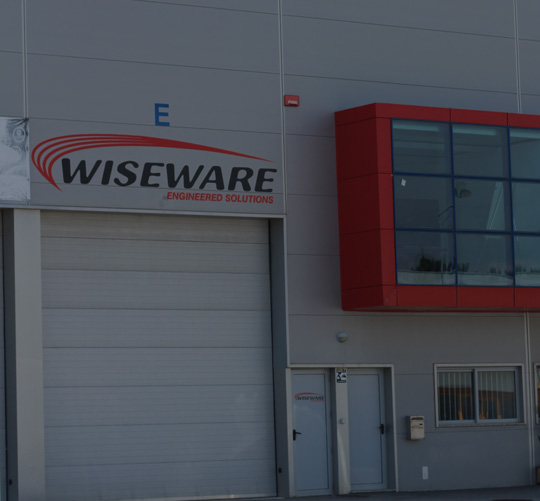
\includegraphics[width=6cm]{figs/wiseware.png}
    \caption[WiseWare Solutions]{Wiseware Solutions}
    \label{fig:company}
\end{figure}

A WiseWare realiza vários serviços como a criação de PCB, montagem de \acs{smt}, inspeção de \acs{smt}, desenho tecnico, cortes 2D/3D a lazer, fresagem, etc.

Apresentam um conjunto de parceiros como a \textit{\ac{ua}}, o \textit{\ac{it}}, a escolha de engenharia da \textit{\ac{um}}, a \textit{inovaria}, entre outros. Como seus clientes estão nomes como a \textit{Adidas}, \textit{Digital Logic}, \textit{Efcom}, grupo \textit{iPesa}, etc.
%\chapter{Entidade de acolhimento}%
\label{chapter:entidade}

A WiseWare Solutions é uma empresa de \acs{randd} localizada na Zona Industrial da Mota Gafanha da Encarnação com a missão de desenvolver soluções inovadores e de alta qualidade para empresas.

A WiseWare é responsável por produzir soluções em áreas como robotica,micro eletronica, inteligencia artificial, comunicações sem fio e muito mais. Aplicaram o seus conhecimentos em projetos de saúde e bem-estar, telemetria, controlo de qualidade, inspeção e automação de sistemas.

\begin{figure}[h!]
	\centering
    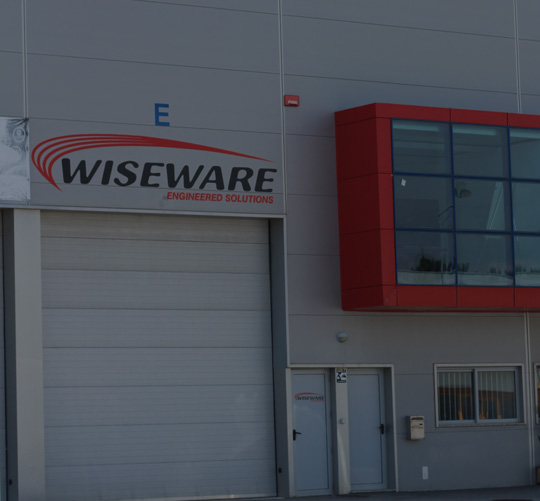
\includegraphics[width=6cm]{figs/wiseware.png}
    \caption[WiseWare Solutions]{Wiseware Solutions}
    \label{fig:company}
\end{figure}

A WiseWare realiza vários serviços como a criação de PCB, montagem de \acs{smt}, inspeção de \acs{smt}, desenho tecnico, cortes 2D/3D a lazer, fresagem, etc.

Apresentam um conjunto de parceiros como a \textit{\ac{ua}}, o \textit{\ac{it}}, a escolha de engenharia da \textit{\ac{um}}, a \textit{inovaria}, entre outros. Como seus clientes estão nomes como a \textit{Adidas}, \textit{Digital Logic}, \textit{Efcom}, grupo \textit{iPesa}, etc.
%\chapter{Plano de trabalho}%
\label{chapter:work-plan}

Antes do estágio começar, foi definido um plano de trabalho que estabelecia os principais objetivos a atingir no decorrer do mesmo, \autoref{fig:work_plan}. Embora este plano represente a base para a realização do estágio, é expectável que, no final, possam existir variações entre o trabalho inicialmente planeado e o efetivamente realizado.

O documento apresenta os objetivos propostos, as atividades a desenvolver para a sua concretização e as horas prevista por atividade. Estes objetivos encontram-se organizados por áreas de trabalho distintas, conforme ilustrado na referida \autoref{fig:work_plan}.

A fase inicial de acolhimento e introdução ao desenvolvimento, com uma previsão de 40 horas, visou a introdução com o ambiente de trabalho e, a aquisição de conhecimentos sobre as tecnologias e ferramentas essenciais usadas pela empresa no processo de desenvolvimento, como \textit{Git}, \textit{Gitlab}, \textit{Jenkins}, o ambiente \textit{Java} e \textit{Svelte}.

Seguiu-se o levantamento de requisitos, também estimado em 40 horas. Este período dedicou-se à aquisição de uma compreensão aprofundada do funcionamento do projeto \textit{aniposture}, nomeadamente dos seus objetivos, estrutura e tecnologias envolvidas.

O estudo e seleção da \textit{\acs{api}} de Mapas constituiu um objetivo crucial, com 120 horas alocadas. Esta tarefa implicou uma análise comparativa das funcionalidades, custos e relação custo-benefício de diversas \acs{api}s de georreferenciação, como \textit{Google Maps} e \textit{Mapbox}, para suportar a tomada de decisão.

Com 120 horas previstas, o desenvolvimento da interface de utilizador, \acs{ui}, centrou-se na implementação gráfica e na integração da \acs{api} de georreferenciação previamente selecionada.

Paralelamente, o desenvolvimento de serviços, com igual carga horária de 120 horas, focou-se na criação de serviços \textit{RESTful} e na implementação de \textit{endpoints} essenciais para o funcionamento do \textit{backend} da aplicação.

A realização de testes funcionais, com uma duração estimada de 24 horas, visou validar o correto funcionamento da aplicação e a sua conformidade com os requisitos definidos.

Por fim, dedicou-se tempo à finalização da escrita do relatório, com uma previsão de 2 horas, ainda no decorrer do período de estágio.
\newline

Este plano de trabalho serviu, portanto, como um guia para a realização do estágio, ao definir as principais tarefas e as suas respetivas metas. A sua existencia foi fundamental para direcionar os esforços, servir como base de comparação e permitir medir o progresso do estágio.

% Antigo

% \begin{enumerate}
%     \item O primeiro objetivo correspondeu à fase de \textit{Acolhimento e introdução ao desenvolvimento}. Esta etapa teve como principal finalidade a minha introdução com as tecnologias e ferramentas utilizadas pela empresa no processo de desenvolvimento.
%     \item O segundo objetivo foi o \textit{Levantamento de requisitos}. Nesta fase, a missão consistiu em adquirir um conhecimento aprofundado sobre o funcionamento do projeto \textit{aniposture}, incluindo os seus objetivos, estrutura, tecnologias envolvidas, entre outros aspetos.
%     \item O terceiro objetivo foi a \textit{Escolher a API de Mapas}. Esta etapa teve como finalidade a realização de um estudo e comparação de funcionalidades, preços e relação custo-beneficio das diferentes \textit{APIs} de georreferenciação. 
%     \item O quarto objetivo correspondeu ao \textit{Desenvolvimento da \acs{ui}}. Esta fase visava a implementação da interface gráfica integrando a \textit{API} de georreferenciação previamente selecionada. 
%     \item O quinto objetivo consistiu o \textit{Desenvolvimento de serviços}. Este objetivo procurava  o desenvolvimento de serviços RESTful e a implementação de endpoints úteis para  o funcionamento do backend da aplicação. 
%     \item O sexto objetivo foi \textit{Testes funcionais}. Esta etapa teve como principal finalidade a realização de testes funcionais de forma a verificar o bom funcionamento da aplicação.
%     \item O setimo e último objetivo foi o \textit{Relatório}. Ainda durante o período de estágio, foram alocadas algumas horas para a redação e finalização do presente relatório.
% \end{enumerate}



%\chapter{Trabalho realizado}
\label{chapter:work-done}

\begin{introduction}
    Neste capítulo irei abordar todo o trabalho desenvolvido durante o período de estágio, organizado em quatro grandes secções. Na primeira farei uma pequena descrição do projeto \textit{aniposture}. Na segunda abordarei o trabalho realizado durante a analise de \textit{APIs} e bibliotecas, incluindo o porque da escolha final de cada uma. A terceira secção visa comentar o trabalho realizado na interface gráfica do projeto \textit{aniposture}. E por fim comentarei o trabalho desenvolvido no respetivo \textit{backend}.
\end{introduction}

\section{Descrição do projeto}\label{sec:project} % Fechada
O projeto \textit{Aniposture} apresenta uma solução inovadora que integra dispositivos inteligentes e tecnologias de análise de dados para monitorar o bem-estar animal e melhorar os processos agropecuários. 

O objetivo consiste em proporcionar uma gestão eficiente e precisa do comportamento dos animais, através de coleiras equipadas com sensores que registam o movimento, medem a temperatura, avaliam a postura e determinem a localização via \acs{gps}. Os módulos de comunicação das coleiras enviam os dados para uma infraestrutura \textit{cloud}, que centraliza e processa a informação.

Cada coleira incorpora uma \textit{IMU}, Unidade de Medição Inercial, com uma frequência de amostragem ajustável, o que permite a recolha de dados sobre a aceleração e a orientação.Desta forma, é possível identificar padrões de movimento e posturas, como estar deitado, em pé ou em movimento. A coleira integra sensores de temperatura que permitem monitorar tanto a temperatura atmosférica como a do temperatura animal. O dispositivo regista igualmente o estado da bateria e emite alertas quando o nível encontra-se baixo. Inclui ainda uma interface \acs{nfc} que possibilita a configuração local dos dispositivos.

A plataforma na \textit{cloud} disponibiliza a informação por meio de uma interface \textit{web}. Entre as funcionalidades incluem-se a visualização do estado das coleiras e o acompanhamento em tempo real das localizações \acs{gps}. A interface apresenta ainda gráficos e filtros por coleira e por período temporal, o que permite consultar a informação de forma rápida e eficaz.

A combinação da tecnologia integrada nas coleiras com a infraestrutura \textit{cloud} coloca o projeto \textit{aniposture} na vanguarda da inovação no sector agropecuário, o que favorece uma gestão mais eficiente e sustentável dos rebanhos.

\section{Análise de bibliotecas}\label{sec:analysis}
Durante este estágio, foram-me atribuídas tarefas de análise e pesquisa, com o objetivo de identificar e selecionar as ferramentas mais adequadas que cumprissem os requisitos necessários para o desenvolvimento da aplicação. Foram, assim, realizadas duas grandes análises: a primeira sobre as \textit{APIs} de georreferenciação e a segunda nas \textit{APIs} de visualização gráfica.

\subsection{APIs georreferenciação} % Fechada
Esta foi uma das primeiras tarefas que foram-me atribuídas durante o estágio. Antes de começar as comparações, foram definidos alguns requisitos fundamentais, nomeadamente a necessidade de \textit{tiles} em satelite, marcadores, bom desempenho com uma elevada quantidade de pontos e desenho de polígonos. Depois de levantados os requisitos, iniciou-se a análise comparativa entre três \textit{APIs} de georreferenciação o \textit{mapbox}, \textit{openlayers} e o \textit{google maps}.

Apesar de partilharem o mesmo objetivo, criação de mapas interativos, as três bibliotecas são consideravelmente diferentes nas suas implementações. 

\subsubsection{\textbf{OpenLayers}}\label{sec:sub_ol} 

\textit{Openlayers} é o biblioteca \textit{free e Open Source} que permite a criação de mapas interativos. Disponibiliza recursos como \textit{raster tiles}, camadas vetoriais e marcadores. Por ser \textit{Open Source}, contem vários \textit{addons} criados pela comunidade que permite alargar as suas funcionalidades. Contudo, apresenta uma linha de aprendizado um pouco mais complexa do que outras alternativas e, por padrão, não contêm  nenhum \textit{tile} em satelite. 

Foram ainda realizados alguns testes com opções de desenho vetorial. No entanto, o que levou o \textit{OpenLayers} não ser o escolhido foi a sua, ainda, baixa integração com \textit{WebGL}, a documentação menos completa em comparação com outras alternativas e a ausência de suporte nativo para mapa com satélite. 

Embora as capacidades de desenho vetorial fossem positivas, apresentava, na altura da análise, algumas limitações para o desempenho exigido em cenários com um elevado volume de dados, como os rastros de localização dos animais. Esta limitação, em conjunto com a complexidade na configuração de funcionalidades essenciais, como as camadas de satélite, e da necessidade de realizar otimizações de forma manual, resultou numa curva de aprendizado mais acentuada e num tempo de desenvolvimento maior. Adicionalmente, a documentação, comparada com outras alternativas, mostrou-se menos completa, o que prolongou a resolução de problemas e a implementação de características específicas. 

Perante este conjunto de constrangimentos, e ao considerar os requisitos de georreferenciação do projeto, optou-se por bibliotecas que demonstraram maior sinergia em termos de performance, facilidade de uso e suporte nativo às funcionalidades pretendidas.

\subsubsection{\textbf{Google Maps}}\label{sec:sub_gm}
O \textit{google maps} é, muito provavelmente, o sistema de mapas mais utilizado e atualizado a nível mundial. Por essa razão, foi considerada a sua utilização, tendo sido analisada a forma como é implementado e as suas funcionalidades. Inicialmente, esta solução revelou-se a mais promissora, uma vez que permite adicionar camadas vetoriais, marcadores, vista em satélite e possui um bom desempenho. 

Ao contrário do \textit{Openlayers}, \ref{sec:sub_ol}, esta é uma solução paga, que apresenta, algumas vantagens como mapas satélite mais atualizados e integração com os serviços da \textit{Google}. Contudo, o maior problema é o seu preço, consideravelmente elevado se formos comprar com outras alternativas. A \textit{Google} permite a utilização da {\textit{Maps JavaScript API}}\cite{google.maps.url} de forma gratuita até 10.000 pedidos mensais. A partir dessa quantidade começam a ser aplicadas cobranças.

%Devido a essa limitação o \textit{google maps} também não foi a solução escolhida.

Embora as suas capacidades técnicas fossem adequadas, a sua integração com outros serviços da \textit{Google} e a qualidade das suas vistas de satélite fossem vantajosas, a estrutura de custos e a incerteza associada ao escalonamento da utilização impediram a sua seleção final. A prioridade recaiu sobre bibliotecas que oferecessem um modelo de licenciamento mais previsível e economicamente sustentável.

\begin{figure}[!h]
	\centering
	\begin{subfigure}[c]{0.45\textwidth}
	\centering
	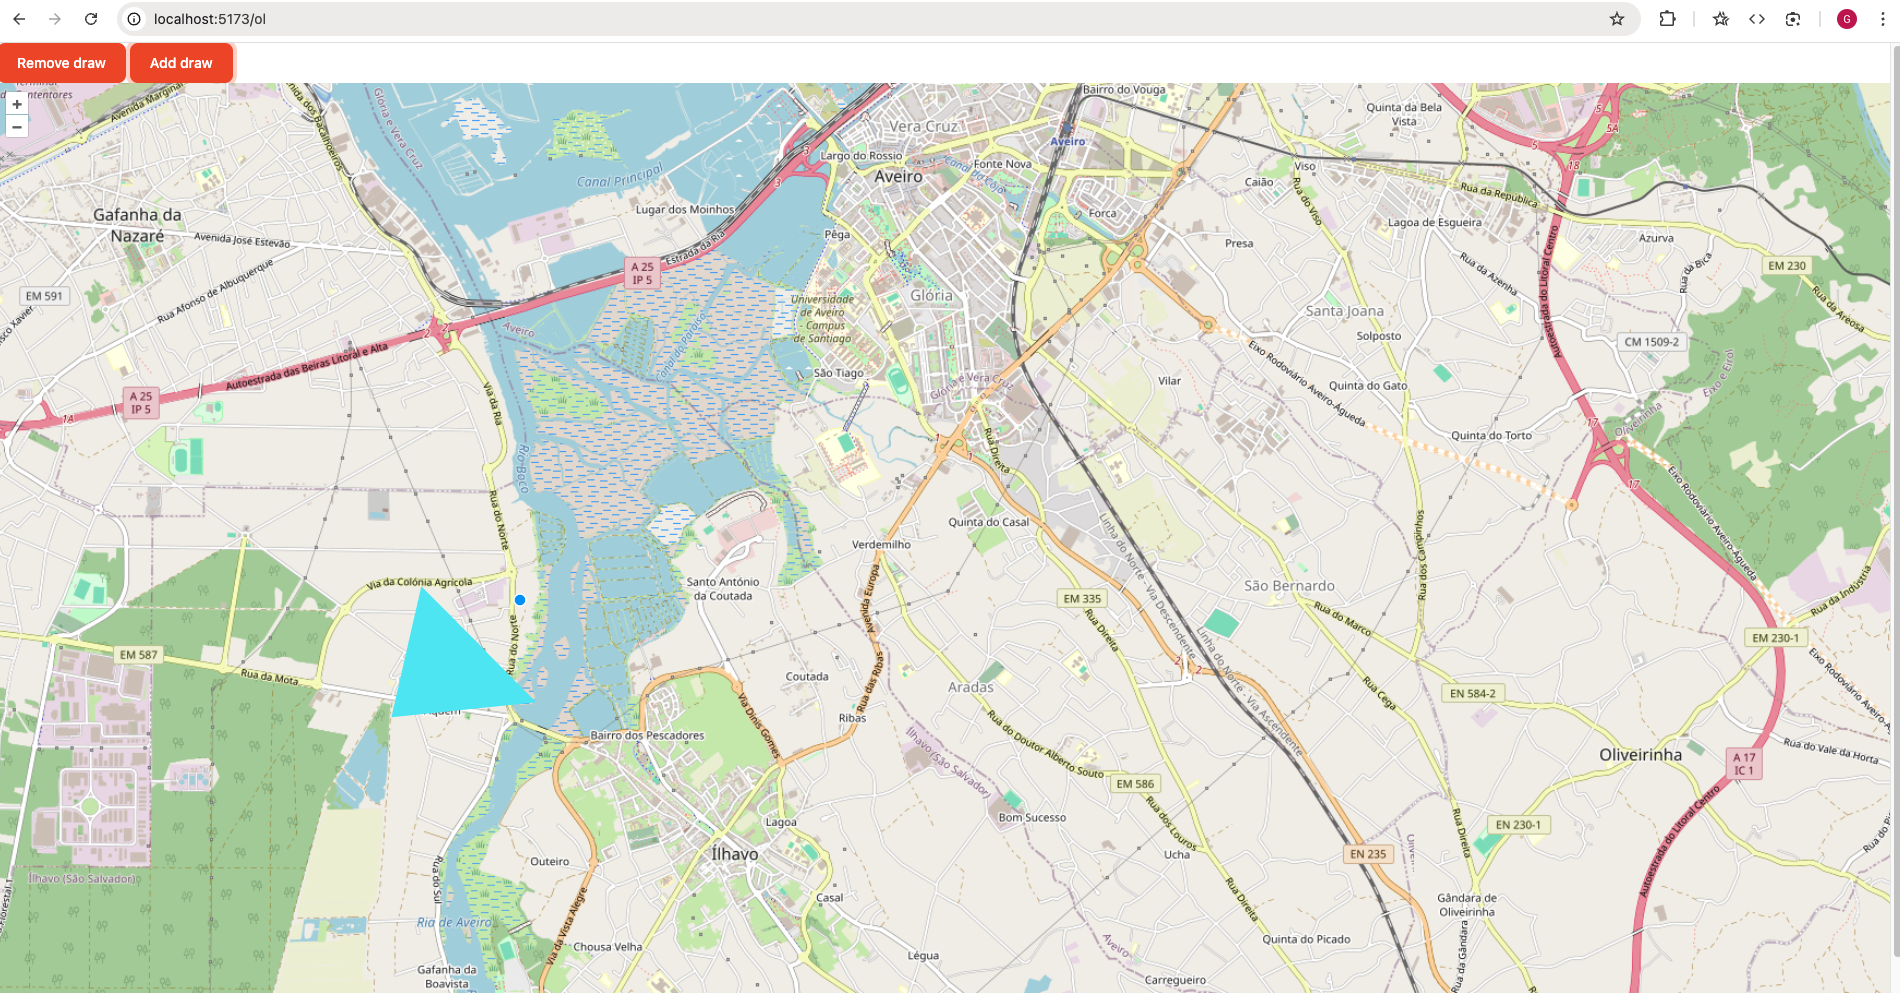
\includegraphics[width=\textwidth]{figs/ol.png}
	\caption{OpenLayers}
	\label{fig:ol}
	\end{subfigure}
	\hfill
	\begin{subfigure}[c]{0.45\textwidth}
		\centering
		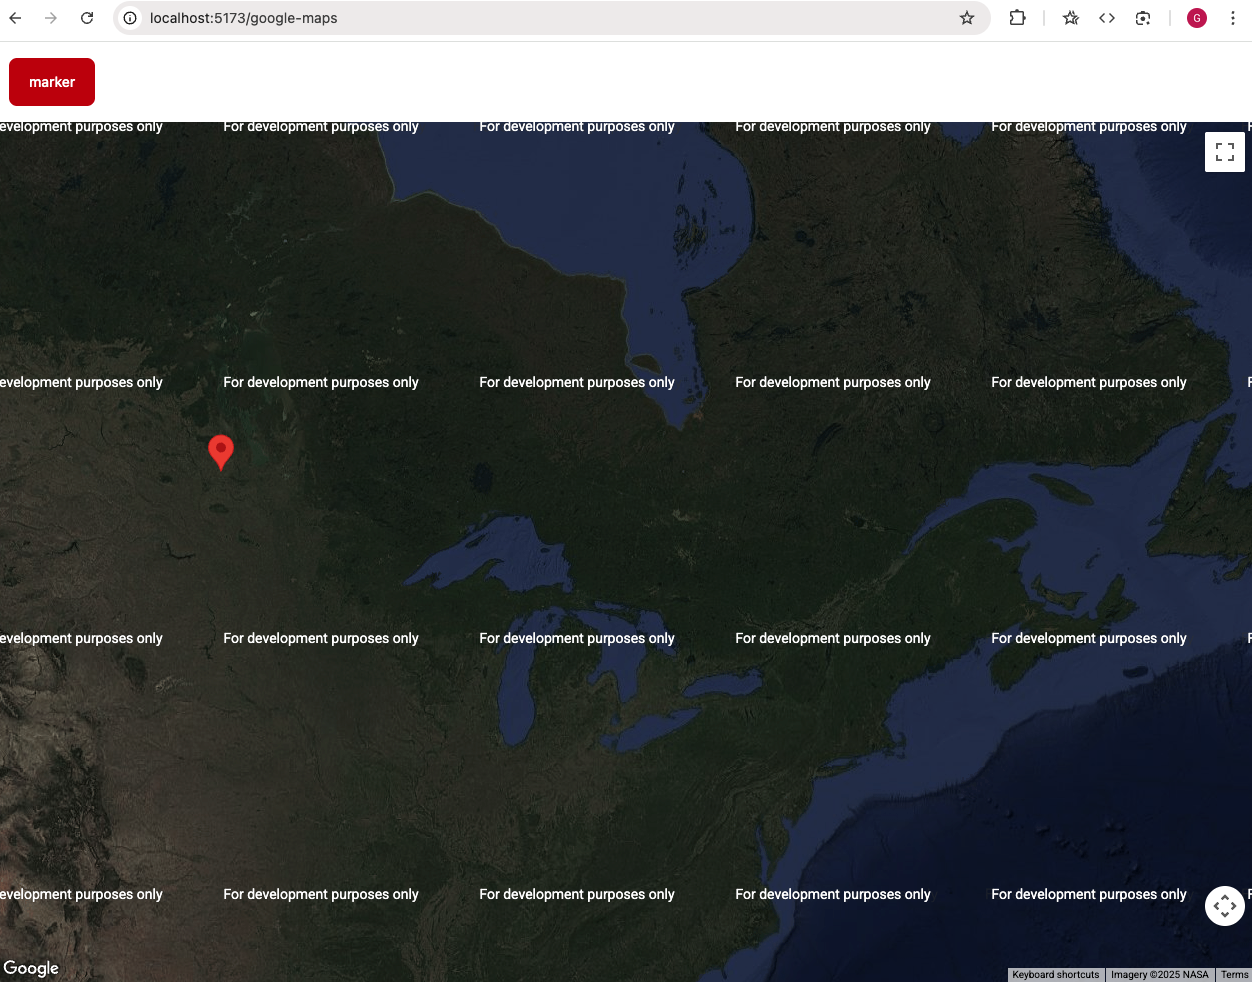
\includegraphics[width=\textwidth]{figs/gm.png}
		\caption{Google Maps}
		\label{fig:gm}
	\end{subfigure}
	\caption{\textit{OpenLayers} \& \textit{Google Maps}}
    \label{fig:1}
\end{figure}

\clearpage
\subsubsection{\textbf{Mapbox}}\label{sec:mapbox} % Fechada
Chegamos, por fim, à opção escolhida: o \textit{Mapbox}. Esta biblioteca revelou-se a melhor entre os dois mundos, implementação inicial simples, utiliza \textit{WebGL} por padrão e disponibiliza vários tipos de \textit{tiles}, incluindo satélite. 

Embora seja uma solução paga, apresenta modelos mais em conta do que a opção da \textit{google}, a versão gratuita, contem um total de 50.000 pedidos por mês. Esta mesma quantidade de pedidos no \textit{google maps} teria um custo de cerca de 280€ mensais. Para atingir um custo parecido no \textit{mapbox}, seria necessário utilizar pelo menos 100.000 pedidos mensais. Para além do fator preço/economico, esta solução, compre todos os requisitos definidos para a nossa aplicação, juntamente de uma documentação bem estruturada.

Tendo em conta todos os requisitos levantados, o \textit{mapbox} cumpre-os de forma exímia. Graças á sua grande comunidade, o \textit{mapbox}, dispõe vários plugins que permitem expandir significativamente as suas funcionalidades, o que acrescenta ainda mais valor à sua escolha como opção para o projeto.

\begin{figure}[h!]
    \centering
    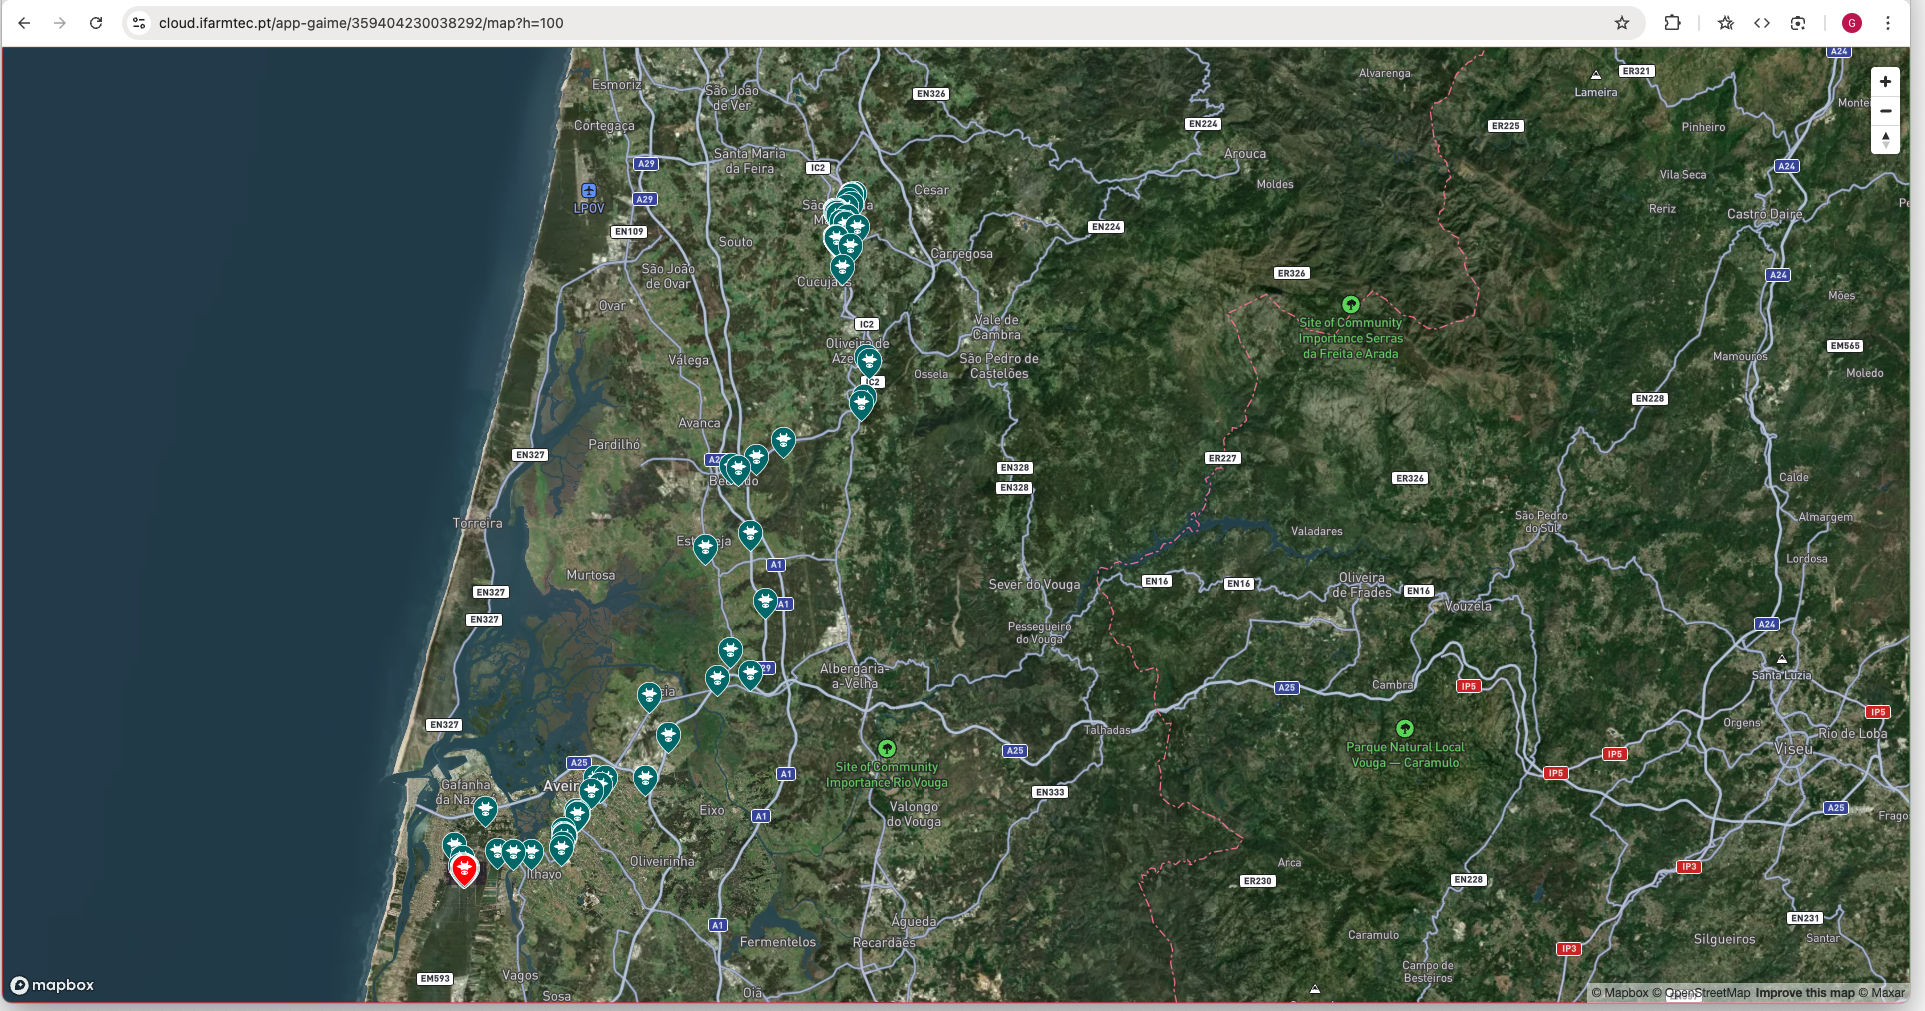
\includegraphics[width=0.8\textwidth]{figs/mapbox.png}
    \caption[Mapbox]{Mapbox}
    \label{fig:mapbox}
\end{figure}

A implementação mais simples com o uso nativo de \textit{WebGL} no \textit{Mapbox} garante não só um desenvolvimento mais rápido, mas também a capacidade de processar e renderizar grandes volumes de dados, tais como os trajetos de múltiplos animais ou o desenho de polígonos para delimitar áreas. Esta performance é crucial para oferecer aos utilizadores uma melhor experiência, mais fluida e em tempo real, permitindo-lhes monitorar os animais de forma detalhada e interativa.

Do ponto de vista económico, a estrutura de preços do \textit{Mapbox} oferece uma vantagem estratégica significativa, o que proporciona uma maior previsibilidade e controlo de custos. Ao juntar a isto, a qualidade da documentação técnica do \textit{Mapbox} facilita a integração, a resolução de problemas e a manutenção do código.


\subsection{APIs de visualização gráfica} % Fechada
Após analise e avaliação das bibliotecas de georreferenciação, realizei uma pequena pesquisa e comparação na área dos gráficos.


\subsubsection{\textbf{D3js}}\label{sec:d3js}
Esta foi a biblioteca identificada pelo orientador, como uma possível opção a implementar. O \textit{d3js} não é uma biblioteca de gráficos tradicional, uma vez que não possui o conceito de "gráficos". Quando visualizamos os dados com o \textit{d3js}, estamos a compor uma variedade de objetos primitivos, como linhas, círculos, retângulos, entre outros. 

Apesar de apresentar um desempenho elevado e permitir um elevado nível de interatividade, a sua utilização é consideravelmente mais complexa que outras alternativas.


\begin{figure}[h!]
    \centering
    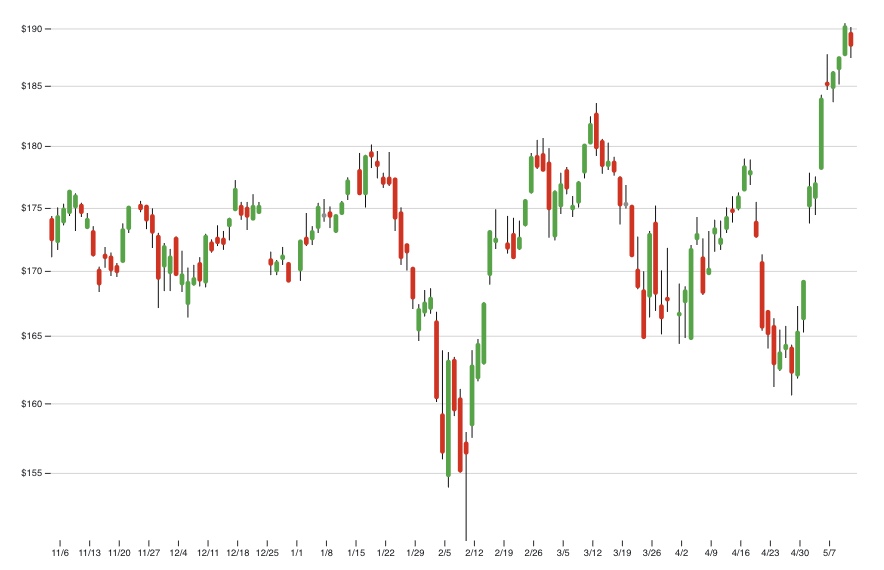
\includegraphics[width=0.7\textwidth]{figs/d3js.png}
    \caption[Gráfico d3js]{Exemplo de gráfico criado com o d3js}
    \label{fig:d3js}
\end{figure}

\subsubsection{\textbf{ChartJs}}\label{sec:chartjs}
O \textit{chartJs} é uma das bibliotecas mais conhecidas e amplamente utilizadas no mundo \textit{JavaScript} para representação de dados.À data atual, conta com mais de \textbf{66 mil} estrelas no \textit{github}\cite{chartJs.github.url} e é regularmente atualizada pela comunidade e pelos seus contribuidores.

Ao contrário do \textit{d3js}, \ref{sec:d3js}, o \textit{chartJs} é consideravelmente mais simples de utilizar. Trata-se de uma biblioteca que incorpora o conceito  de "gráfico", permite a visualização da informações em 8 estilos diferentes, sendo ainda responsivo. 

No entanto, essa mesma simplicidade pode ser vista como uma limitação: os gráficos, por padrão, oferecem poucos funcionalidades além da visualização básica dos informação.

\begin{figure}[h!]
    \centering
    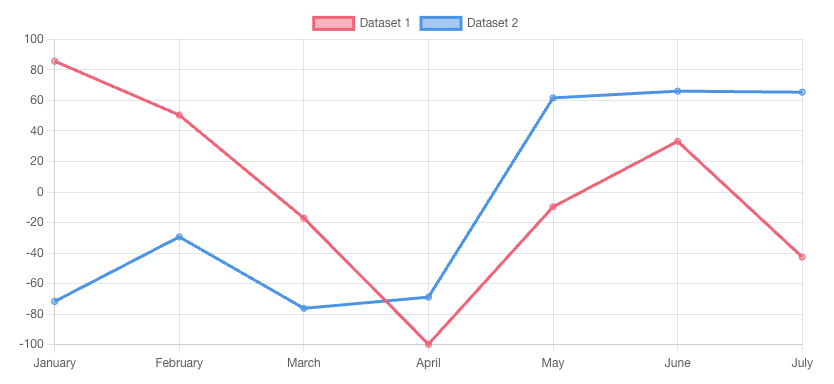
\includegraphics[width=0.8\textwidth]{figs/chartJs.png}
    \caption[Gráfico chartJs]{Exemplo de gráfico criado com o chartJs}
    \label{fig:chartjs}
\end{figure}

\subsubsection{\textbf{Echarts}}\label{sec:echarts}
\textit{Apache Echarts} é uma biblioteca gratuita, desenvolvida no âmbito da fundação \textit{Apache}, que apresenta caracteristicas similares ao chartJs. Suporta mais de 20 tipos diferentes de gráficos, é responsivo e permite a renderização de até 10 milhões de dados em tempo real.

\begin{figure}[h!]
    \centering
    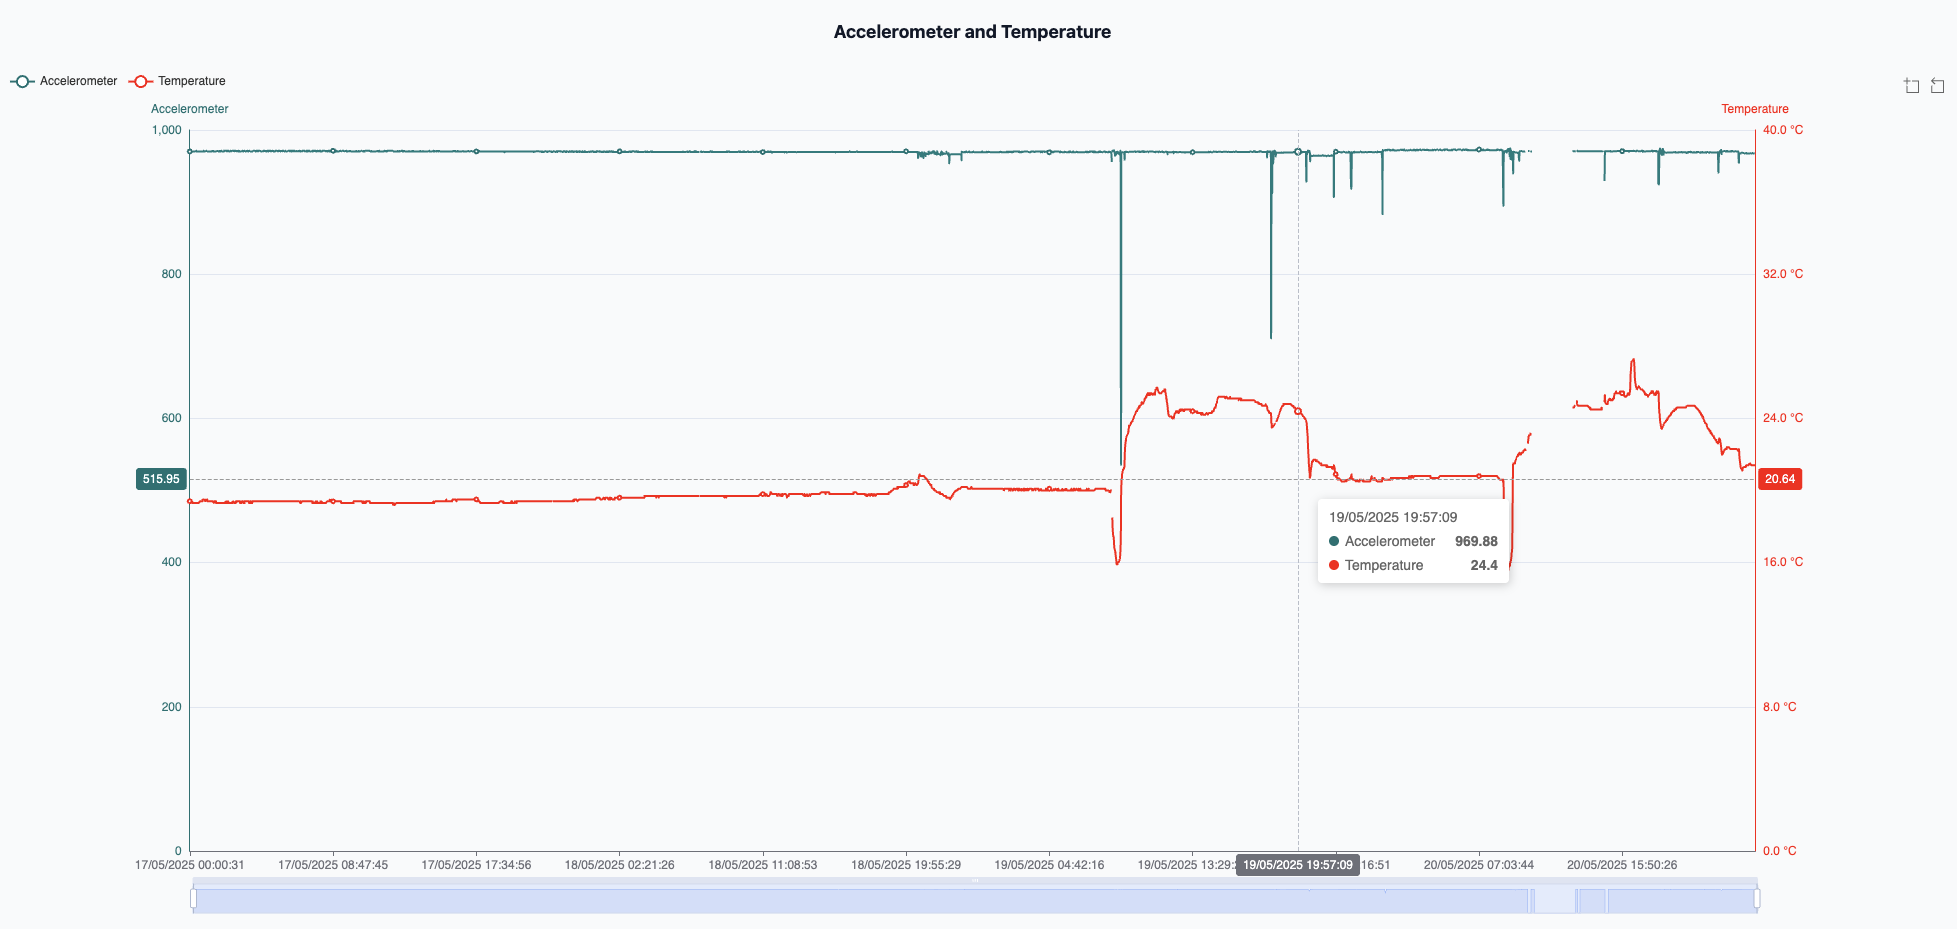
\includegraphics[width=0.8\textwidth]{figs/echarts.png}
    \caption[Gráfico Apache Echarts]{Exemplo de gráfico criado com Echarts}
    \label{fig:echarts}
\end{figure}

O \textit{Apache Echarts} foi a solução escolhida para integrar no projeto, não apenas por apresentar um maior número de opções de visualização de dados, mas também pelas suas pelas suas funcionalidades nativas e pela elevada performance a carregar uma grandes volumes de dados. 

\clearpage
\section{Interface gráfica}\label{sec:frontend}
Nesta fase, será abordado com detalhes todo o trabalho realizado no \textit{frontend}/interface gráfica da aplicação, incluindo as dificuldades encontradas, conhecimentos adquiridos e as tarefas realizadas durante o desenvolvimento.  

\subsection{Svelte 5}\label{sec:svelte5} % Fechada
Durante a fase de desenvolvimento, esta foi das primeiras tarefas que foram-me atribuídas. No último trimestre de 2024, a equipa responsável pelo \textit{svelte} lançou uma nova versão, que alterou conceitos fundamentais da \textit{framework}. Fui, então, encaminhado a aprender esta nova versão, testar as novas funcionalidades, compreender as principais alterações e analisar o processo de atualização de um projeto desenvolvido na versão 4 para a versão 5 do \textit{svelte}.  

O \textit{svelte} 5 introduziu um novo conceito denominado \textit{runes} (runas), que consistem num mecanismo para declarar estado de reatividade. As runas são símbolos que influenciam o compilador do \textit{svelte}, permitem ao programador definir, de forma explícita, quais objetos são reativos e quais não são, \autoref{fig:svelte5}. 

Nas versões anteriores, o \textit{svelte} tornava todos os objetos reativos por padrão, isto dificultava a perceção de quais objetos podiam, efetivamente, provocar alterações na interface gráfica.

Estas mudanças representam uma alteração significativa na forma como criavamos código em \textit{svelte}. A nova abordagem, removeu a sintaxe do \textit{svelte} 4, \autoref{fig:svelte4}, que, muitas das vezes, era confusa, já que a mesma expressão podia realizar ações diferentes. Com a introdução da nova sintaxe, cada uma das ações realizas é bem definida, o que torna o código mais previsível e fácil de manter. 

\begin{figure}[!h]
	\centering
	\begin{subfigure}[c]{0.45\textwidth}
		\centering
		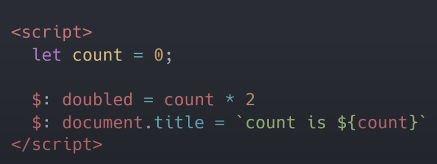
\includegraphics[width=\textwidth]{figs/svelte4.png}
		\caption{Exemplo \textit{Svelte} 4}
		\label{fig:svelte4}
	\end{subfigure}
	\hfill
	\begin{subfigure}[c]{0.45\textwidth}
		\centering
		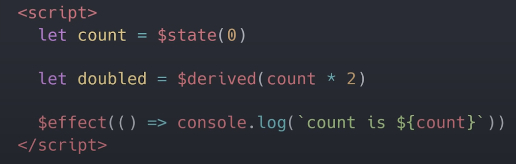
\includegraphics[width=\textwidth]{figs/svelte5.png}
		\caption{Exemplo \textit{Svelte} 5}
		\label{fig:svelte5}
	\end{subfigure}
	\caption{Diferenças \textit{Svelte} 4 e 5}
\end{figure}

Uma das alterações introduzidas nesta nova versão do \textit{svelte} foi a forma como passamos elementos para dentro dos componentes. 

Na versão anterior, utilizava-se a palavra-chave \textit{export}, o que permitia declarar propriedades em qualquer parte do componente. Essa flexibilidade, embora útil, podia tornar o código menos organizado e mais difícil de compreender. Na nova versão, todos os elementos recebidos pelo componente são definidos num único local, o que promove uma estrutura mais clara e facilita a leitura e manutenção do código. Ver \autoref{fig:propsSvelte}.

\begin{figure}[h!]
    \centering
    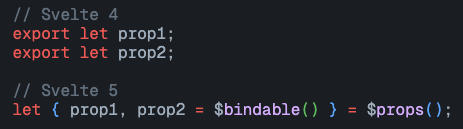
\includegraphics[width=0.8\textwidth]{figs/props.png}
    \caption{Exemplo \textit{props svelte}}
    \label{fig:propsSvelte}
\end{figure}

Depois de familiarizar-me com os novos conceitos introduzidos no \textit{svelte} 5, iniciei a modificação e criação novos componentes nesta versão. Os dois conceitos mais importes, e os que exigiram mais tempo a compreender foram o \textit{\$derived} e o \textit{\$effect}.

O \textbf{\textit{\$derived}} é uma runa utilizada para definir uma variavel derivada. Ou seja, cria-se uma nova variavel cujo o valor é automaticamente atualizado com base numa expressão, sempre que ocorre alguma alteração noutra variavel, \autoref{fig:svelte5}.

Já o \textbf{\textit{\$effect}} é uma função que é executada sempre que um determinado estado é atualizado. Esta runa pode ser utilizada, por exemplo, para chamar biblioteca externas, desenhar elementos num canvas ou realizar pedidos à rede, \autoref{fig:svelte5}.

\begin{figure}[!h]
	\centering
	\begin{subfigure}[c]{0.45\textwidth}
		\centering
		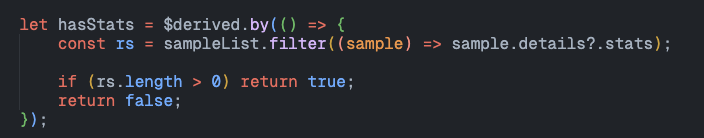
\includegraphics[width=\textwidth]{figs/derived.png}
		\caption{Exemplo \textit{\$derived}}
		\label{fig:derived}
	\end{subfigure}
	\hfill
	\begin{subfigure}[c]{0.45\textwidth}
		\centering
		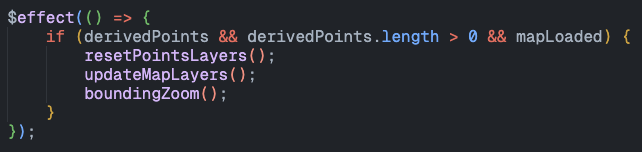
\includegraphics[width=\textwidth]{figs/effect.png}
		\caption{Exemplo \textit{\$effect}}
		\label{fig:effect}
	\end{subfigure}
	\caption{\textit{\$derived \& \$effect}}
    \label{fig:derived_effect}
\end{figure}

Na \autoref{fig:derived_effect}, podemos ver um exemplo um pouco mais complexo da utilização das runas \textit{\$derived e \$effect}. 

No caso do \textit{\$derived}, a variavel \textit{hasStats} é atualizada sempre que ocorrem alterações no \textit{array sampleList}. Já o \textit{\$effect} executa todas as funções chamadas no seu interior sempre que o mapa está carregado e a variavel \textit{derivedPoints} é alterada.

\clearpage
\subsection{Tecnologias fundamentais}\label{sec:tec_fund_ani} % Fechada

Nesta secção irei comentar um pouco sobre as outras tecnologias que existem no projeto \textit{aniposture}. 

\subsubsection{\textbf{Tailwind}}
O \textit{tailwind} é uma \textit{framework} css que permite construir interfaces diretamente no \textit{HTML}, através da utilização de classes pré definidas. Esta abordagem promove rapidez e consistência no design, o que reduz necessidade de escrever \textit{CSS} personalizado.

Esta foi a minha primeira experiencia com tailwind. Encontrei algumas dificuldades nas primeiras semanas, sobretudo por ainda não compreender totalmente o seu conceito nem as suas classes pré definidas. No entanto, após ultrapassar esta fase de adaptação, consegui desenvolver interfaces de forma mais rápida e prática.

\begin{figure}[h!]
    \centering
    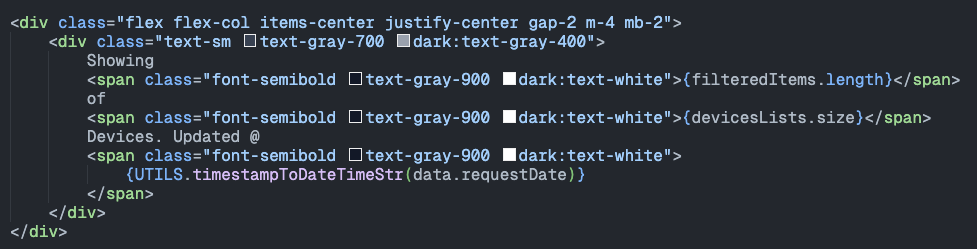
\includegraphics[width=0.8\textwidth]{figs/tailwind.png}
    \caption{Exemplo de interface criada com \textit{tailwind}}
    \label{fig:tailwind}
\end{figure}

\subsubsection{\textbf{Flowbite svelte}}
O \textit{flowbite} é uma biblioteca de componentes baseada em \textit{tailwind}, que tem como objetivo acelerar e simplificar a criação de interfaces. Esta fornece um vasto conjunto de componentes prontos a usar, como tabelas, botões, modais, entre outros. A utilização destes componentes contribui para uma interface mais uniforme e coerente.

\begin{figure}[h!]
    \centering
    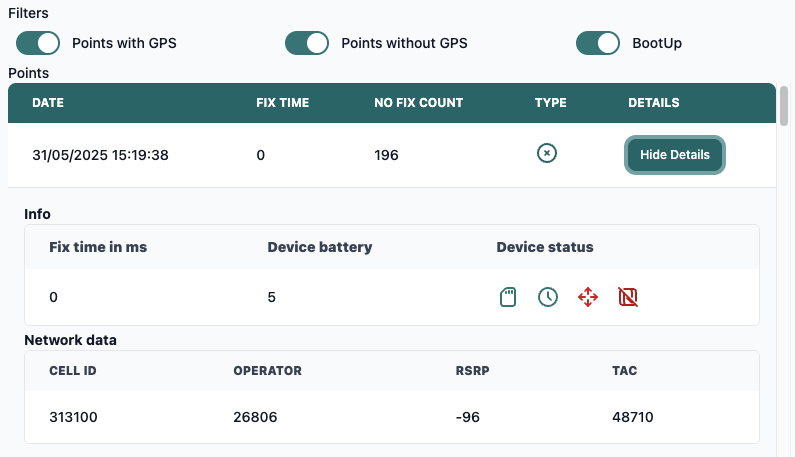
\includegraphics[width=0.7\textwidth]{figs/flowbite.png}
    \caption{Interface com componentes \textit{flowbite}}
    \label{fig:flowbite}
\end{figure}

\clearpage 
\subsection{Alterações no \textit{design system}} % Fechada
Uma das tarefas que executei durante o desenvolvimento deste projeto foi a reformulação da interface, alteração que abrangeu todas as páginas da aplicação.

Para tornar essa reformulação possível, alterei o tema principal. O tema anterior, gerado automaticamente pelo \textit{tailwind} a partir de uma única cor, originou uma paleta cromática que se afastava da identidade visual pretendida para a aplicação.

A \autoref{fig:tailwindGeneratedColors} mostra que as tonalidades mais claras da aplicação apresentavam um azul claro que não combinavam com as restantes cores. Para corrigir essa incoerência, alterei a paleta cromática para um sistema de sombras, mantendo a mesma cor base em variações mais claras e mais escuras. O novo esquema confere um aspeto mais agradável à seleção de botões, às colunas das tabelas, aos realces e aos demais elementos.

Esta mudança de paleta assegura que a interface respeite a identidade visual definida. A cor base mantém-se, mas apresenta-se em sombras progressivamente mais claras e mais escuras, o que gera uma hierarquia visual consistente. Os componentes que antes exibiam um azul claro passam a integrar-se no conjunto cromático, o que melhora a leitura e a navegação. O resultado oferece uma experiência mais coesa e agradável para o utilizador.

Foram também efetuadas alterações às bibliotecas de ícones. Anteriormente, a aplicação dispunha de uma biblioteca com um número reduzido de ícones, fator que limitava as possibilidades de desenvolvimento. Instalei uma nova biblioteca, \textit{Tabler}\footnote{\href{https://tabler.io/icons}{Tabler - https://tabler.io/icons}}, que apresenta uma vasta gama de opções.

Com o objetivo de tornar a interface mais harmoniosa, introduziram-se alterações que permitem a várias páginas reutilizar componentes, quer do \textit{flowbite}, quer desenvolvidos internamente.

Esta abordagem aumenta a consistência visual e reduz o esforço necessário de desenvolvimento, ao evitar duplicação de código e simplificar a manutenção. Como resultado, a aplicação apresenta um aspeto mais uniforme e permite atualizações mais rápidas no futuro.

\begin{figure}[!h]
	\centering
	\begin{subfigure}[c]{0.45\textwidth}
		\centering
		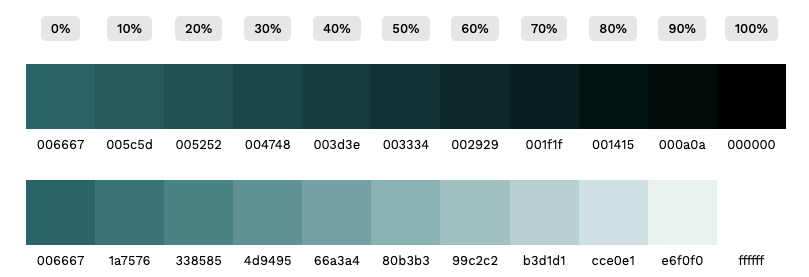
\includegraphics[width=\textwidth]{figs/shades.png}
		\caption{Cores geradas por sombra}
		\label{fig:shadesColors}
	\end{subfigure}
	\hfill
	\begin{subfigure}[c]{0.45\textwidth}
		\centering
		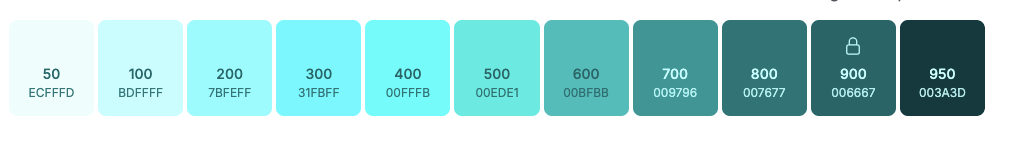
\includegraphics[width=\textwidth]{figs/tailwindGeneratedColors.png}
		\caption{Cores geradas pela tailwind}
		\label{fig:tailwindGeneratedColors}
	\end{subfigure}
	\caption{Sistemas de cores}
    \label{fig:colorSystem}
\end{figure}

\subsection{Componente Mapa}\label{sec:map_comp} % Fechada
Um dos trabalhos mais complexos nesta fase da interface foi a implementação do mapa. Trata-se de um elemento com caracteristicas especiais, que exige funcionalidades como o carregamento de pontos, executar ações ao detetar cliques, carregar \textit{layouts}, atualização automatica de novas informações, desenho de elementos, entre outros. 

Um dos pontos mais importantes durante o desenvolvimento deste componente foi garantir que os dados fossem carregados e atualizados automaticamente. Este aspeto revelou-se particularmente importante devido à arquitetura \textit{multi tenant} do projeto. Ao escolher um novo \textit{tenant}, todas as informações tinham de ser limpas e substituídas por novas. Para atingir este objetivo, foram utilizadas várias ferramentas do \textit{svelte 5}, \autoref{sec:svelte5}.

\subsubsection{\textbf{Layers (Camadas)}}\label{sec:layers}
As \textit{Layers}, ou camadas, são componentes principais em qualquer sistema de mapas. O \textit{mapbox} permite a adição de diversas \textit{camadas} ao mapa, como elementos vetoriais, simbolos, imagens \textit{raster}, modelos 3D, entre outros. Estas camadas permitem representar diferentes tipos de dados geográficos e visuais, sendo fundamentais para a construção de mapas interativos.

Na criação deste componente, foram adicionadas duas camadas para cada tipo de animal existente. Uma das camadas é responsável por mostrar todos os elementos, enquanto a outra exibe apenas os elementos selecionados.

\begin{figure}[!h]
	\centering
	\begin{subfigure}[c]{0.40\textwidth}
		\centering
		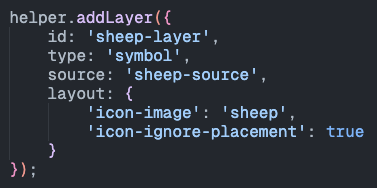
\includegraphics[width=\textwidth]{figs/layer.png}
		\caption{Camada de elementos}
		\label{fig:layer}
	\end{subfigure}
	\hfill
	\begin{subfigure}[c]{0.40\textwidth}
		\centering
		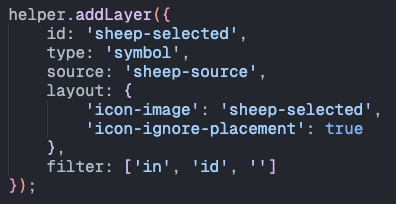
\includegraphics[width=\textwidth]{figs/selected_layer.png}
		\caption{Camadas de elementos selecionados}
		\label{fig:selected_layer}
	\end{subfigure}
	\caption{Camadas}
    \label{fig:layers}
\end{figure}

Como ilustrado na \autoref{fig:layer}, na camada correspondente a todos os elementos é carregada a informação através da fonte \textit{sheep-source}, sendo os elementos posteriormente carregados no mapa. Já a camada \textit{sheep-selected} apenas apresenta os elementos quando o filtro correspondente está ativado. Essa seleção ocorre através do evento \textit{on click}, que identifica o ponto naquela coordenada. Após seleção, o \textit{svelte} atualiza automaticamente os pontos no mapa. \autoref{fig:mapLayersUpdate}.

\begin{figure}[!h]
	\centering
	\begin{subfigure}[c]{0.45\textwidth}
		\centering
		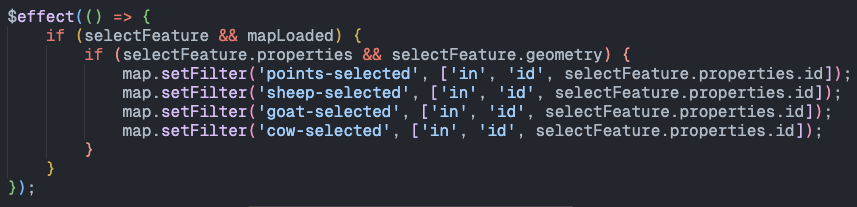
\includegraphics[width=\textwidth]{figs/setfilter.png}
		\caption{Selecionar filtros}
		\label{fig:updateMapSelected}
	\end{subfigure}
	\hfill
	\begin{subfigure}[c]{0.45\textwidth}
		\centering
		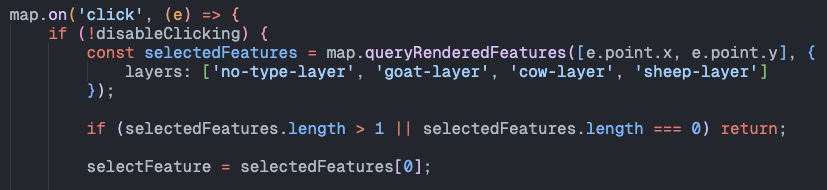
\includegraphics[width=\textwidth]{figs/mapClick.png}
		\caption{\textit{Map onClick}}
		\label{fig:mapClick}
	\end{subfigure}
	\caption{Atualizar pontos selecionados no mapa}
    \label{fig:mapLayersUpdate}
\end{figure}

\subsubsection{}\label{sec:geoJsonConverter}
Uma das funcionalidades que tive de implementar, de forma a facilitar a gestão dos polígonos e dos pontos no mapa, foi a tradução de todos os pontos das camadas para \textit{geoJson}\cite{rfc7946}. Esta conversão, de pontos para \textit{geoJson}, formata toda a informação num padrão reconhecido por múltiplos sistemas. Desta forma, é possível editar e exibir a informação, independentemente da fonte e do formato de origem dos dados.

\begin{figure}[!h]
	\centering
	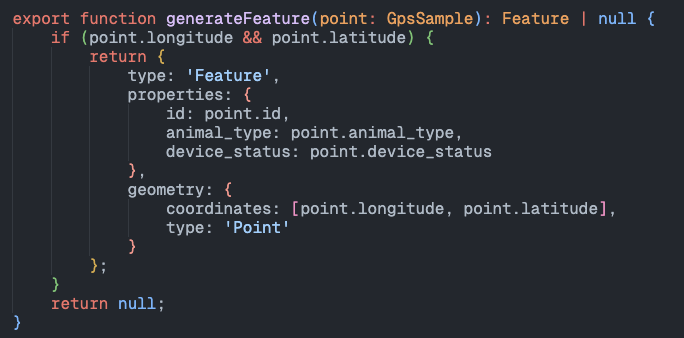
\includegraphics[width=0.55\textwidth]{figs/generateFeature.png}
	\caption{Função \textit{generateFeature}}
	\label{fig:generateFeature}
\end{figure}

No nosso caso, extraímos a latitude e longitude armazenadas nos pontos e convertemos-las numa lista de pontos \textit{geoJson}. Uma das vantagens do \textit{geoJson} é a possibilidade de associar propriedades a cada ponto, que podem ser acedidas posteriormente, ao clicar num ponto. Após gerar cada uma das \textit{features} a partir dos pontos e inseri-las nas camadas corretas, \autoref{fig:pushFeatures}, procedemos à atualização de todas as \textit{sources} do mapa de forma a carregar os novos dados, \autoref{fig:updateSources}.

% Concat não faz sentido aqui. O concat faz referencia ao desenho de poligonos, o facto de contenarmos features que desenhamos e features que já estão no mapa.
\begin{figure}[!h]
	\centering
	\begin{subfigure}[c]{0.45\textwidth}
		\centering
		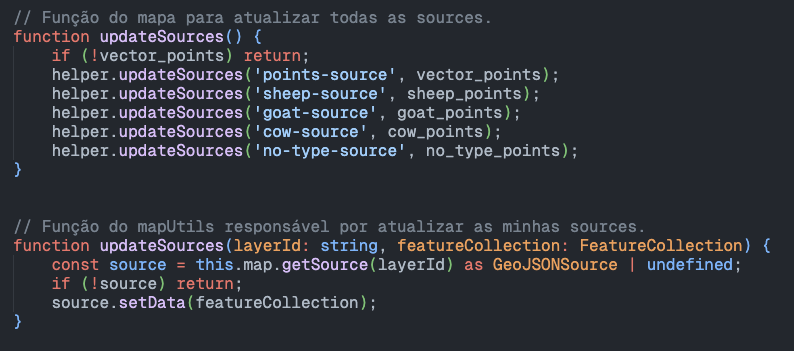
\includegraphics[width=\textwidth]{figs/updateSources.png}
		\caption{Atualizar \textit{sources} do mapa}
		\label{fig:updateSources}
	\end{subfigure}
	\hfill
	\begin{subfigure}[c]{0.35\textwidth}
		\centering
		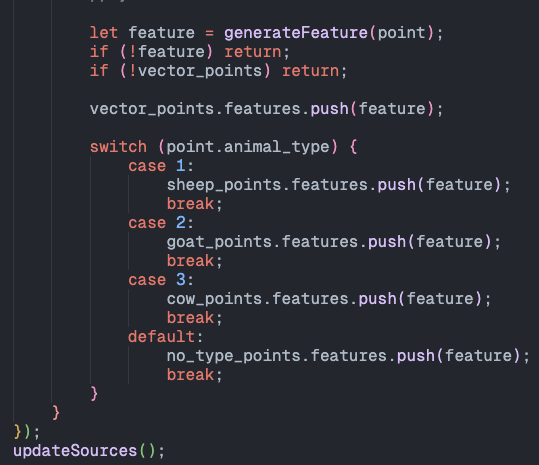
\includegraphics[width=\textwidth]{figs/pushFeatures.png}
		\caption{Adicionar features às layers}
		\label{fig:pushFeatures}
	\end{subfigure}
	\caption{Atualizar e gerar \textit{geoJson features}}
    \label{fig:updateFeatures}
\end{figure}

\clearpage
\subsubsection{\textbf{Marcadores}}\label{sec:markers}
Antes da utilização das camadas vetoriais, descritas na \ref{sec:layers}, foram realizados alguns testes com os marcadores nativos do mapbox. 

Um marcador é uma representação visual de uma coordenada especifica no mapa. Estes marcadores são elementos \textit{html} inseridos no \textit{\acs{dom}} da página, \autoref{fig:markers}. Devido ao baixo desempenho, esta abordagem revela-se inviavel quando se pretende representar mais do que algumas dezenas de pontos. Por esta razão, decidi abandonar esta solução e adotar as camadas vetoriais para a visualização de grandes volumes de dados.

\begin{figure}[h!]
    \centering
    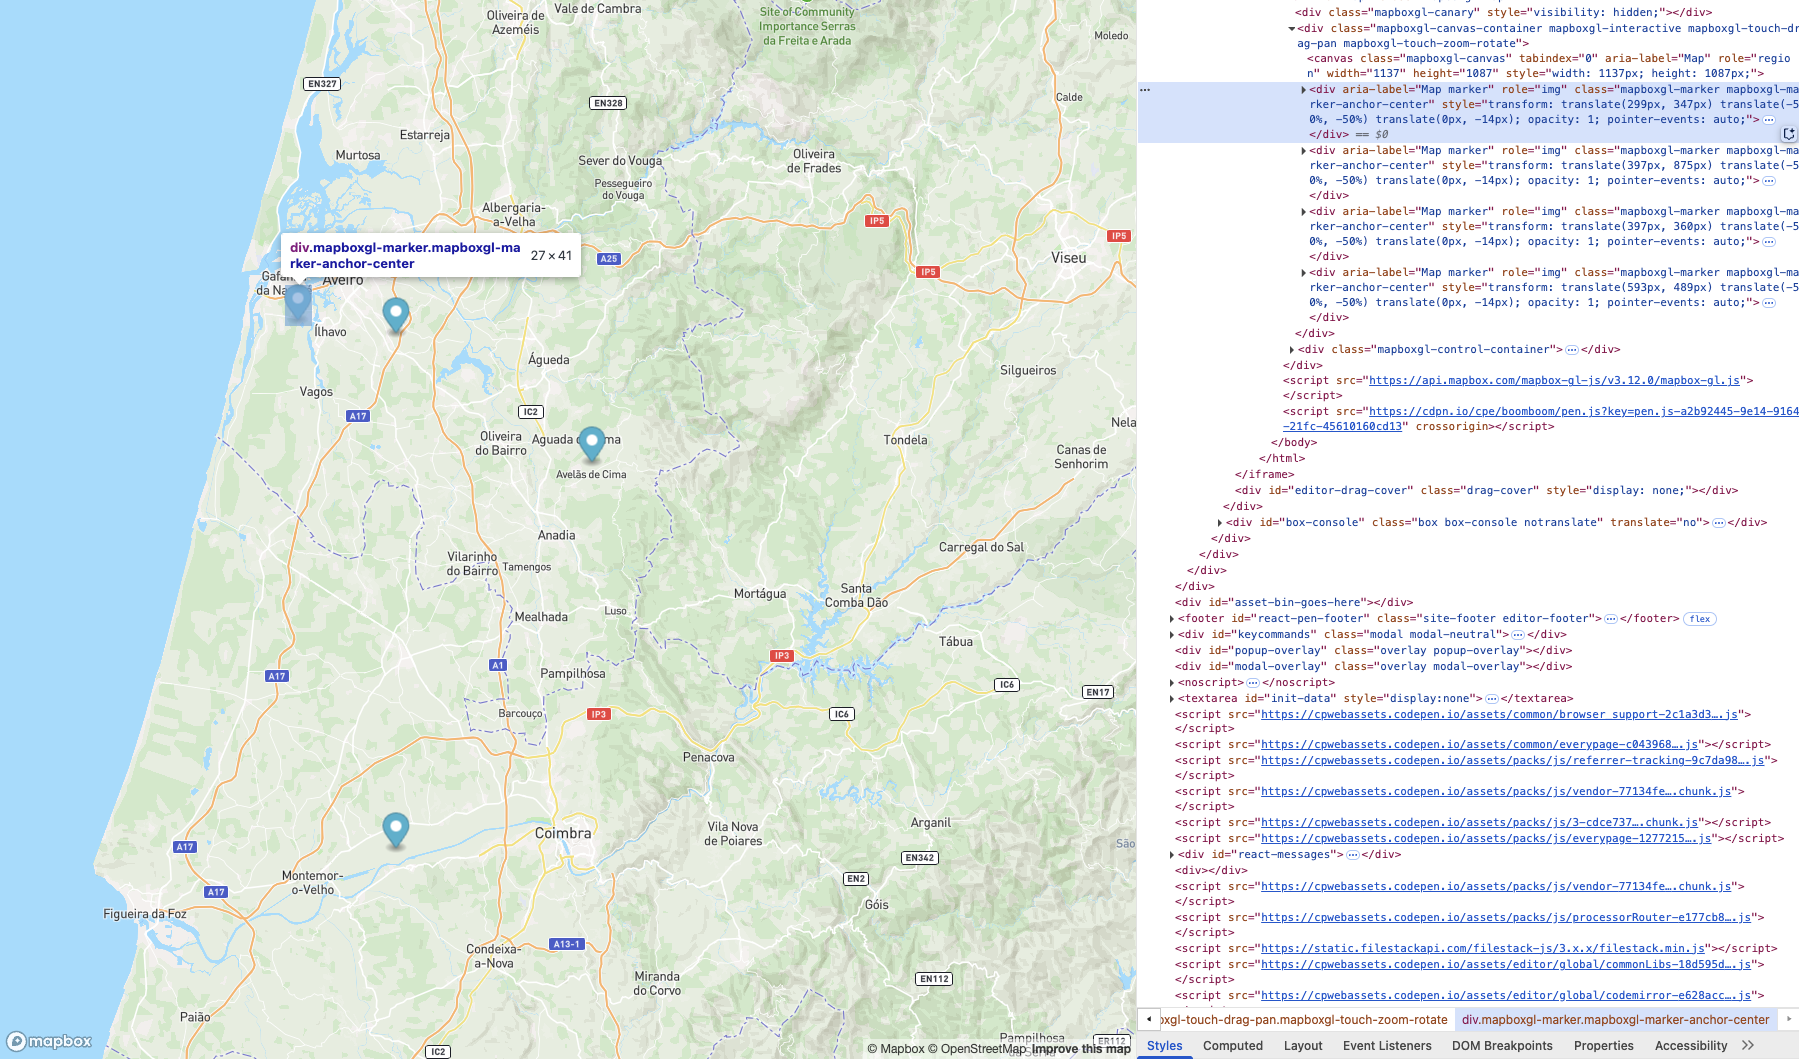
\includegraphics[width=0.6\textwidth]{figs/markers.png}
    \caption{Exemplo de marcadores}
    \label{fig:markers}
\end{figure}


\subsubsection{\textbf{\textit{Map Utils}}}\label{sec:mapUtils}
Para facilitar a criação do mapa e simplificar o desenvolvimento de novos sistemas, foram desenvolvidas algumas classes e interfaces que abstraem e organizam as funcionalidades necessárias. Algumas dessas estruturas podem ser observadas na \autoref{fig:mapUtils}.

\begin{figure}[!h]
	\centering
	\begin{subfigure}[c]{0.30\textwidth}
		\centering
		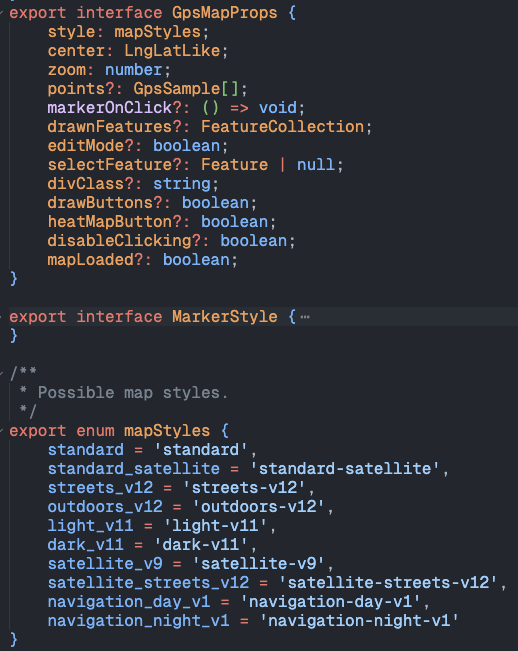
\includegraphics[width=\textwidth]{figs/interfaces.png}
		\caption{\textit{Map Interfaces}}
		\label{fig:mapIntefaces}
	\end{subfigure}
	\hfill
	\begin{subfigure}[c]{0.40\textwidth}
		\centering
		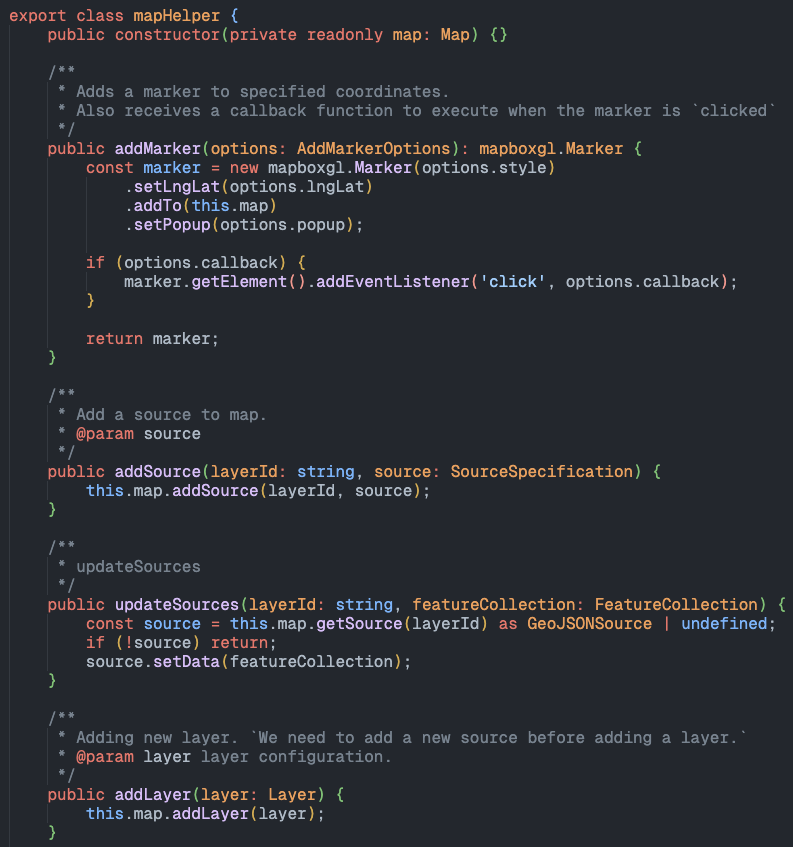
\includegraphics[width=\textwidth]{figs/mapClasses.png}
		\caption{\textit{Map classes}}
		\label{fig:mapClasses}
	\end{subfigure}
	\caption{\textit{Map utils}}
    \label{fig:mapUtils}
\end{figure}


\clearpage
\subsubsection{\textbf{Desenho de poligonos}}\label{sec:polyDraw}
Uma das funcionalidades mais interessantes que desenvolvi foi a implementação de um sistema de desenho e edição de poligonos sobre o mapa.

Durante a pesquisa de funcionalidades semelhantes, deparei-me com uma ferramenta que aproxima-se com a nossa ideia para esta implementação. Para concretizar esta parte da aplicação, inspirei-me no \textit{geojson.io}\footnote{\href{https://geojson.io/}{geojson.io - https://geojson.io/}}. Esta é uma ferramenta \textit{online}, frequentemente utilizada para verificar conteúdos \textit{geojson} e efetuar pequenas alterações.

Esta funcionalidade foi implementada em cima de um \textit{plugin} criado pela comunidade, \textit{mapbox-gl-draw}\cite{mapbox.docs.url}, que permite adicionar funcionalidades de desenho diretamente sobre o mapa. Um dos elementos que deram mais esforço na implementação desta funcionalidade foi a componente de edição. 

Este permite ao utilizador remover, mover, aumentar e diminuir poligonos desenhados. Foram igualmente realizadas alterações no \textit{plugin} de desenho, de modo a adaptar toda a sua interface, cores e opções, garantindo a consistência visual e funcional com o restante da aplicação, \autoref{fig:drawPoly}.

\begin{figure}[h!]
    \centering
    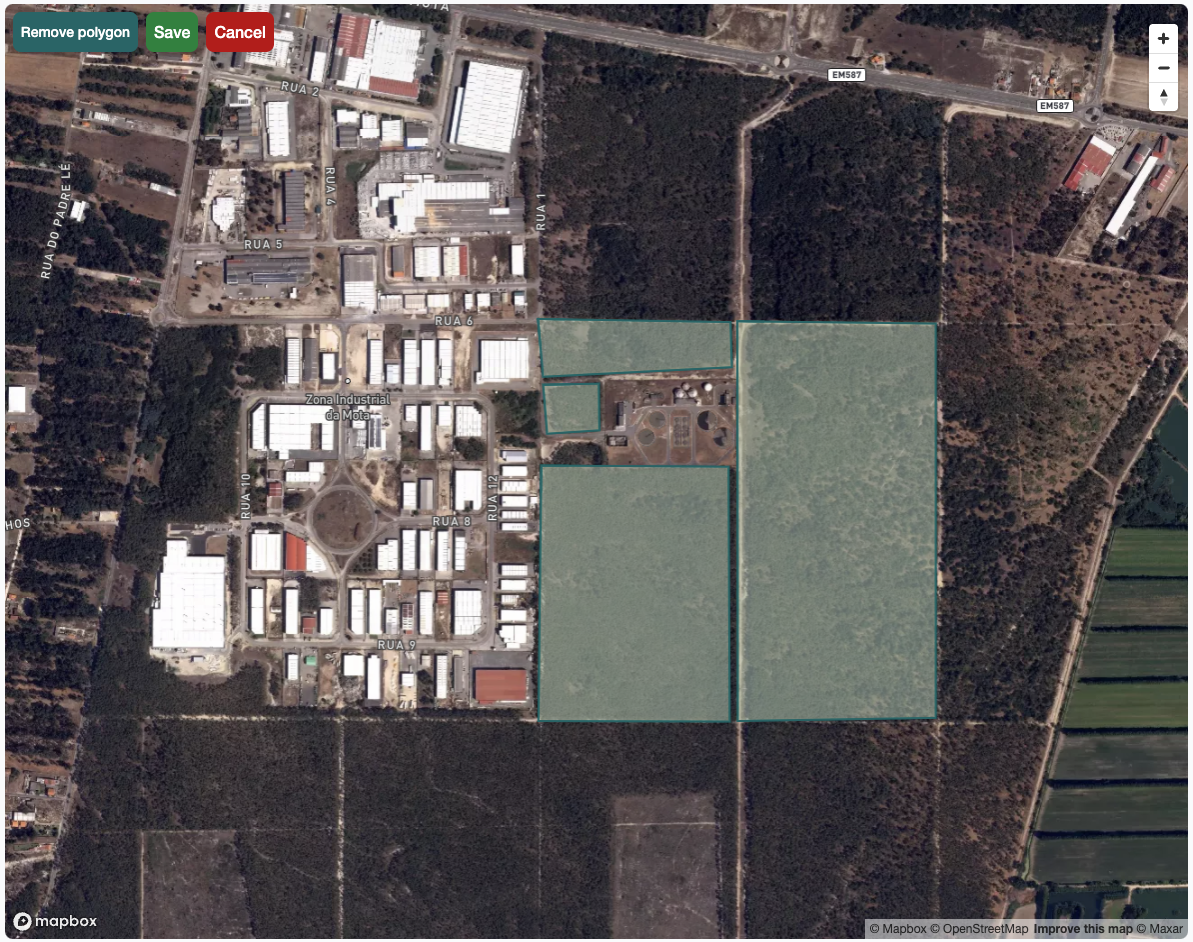
\includegraphics[width=0.55\textwidth]{figs/draw.png}
    \caption{Desenhar polígonos}
    \label{fig:drawPoly}
\end{figure}

%TODO Comentar sobre os problemas encontrados ao criar este sistema

O sistema funciona conforme representado na \autoref{fig:flowchartDraw}. Esta abordagem revelou-se a mais prática e eficiente para desenvolver a funcionalidade de desenho e edição de poligonos. Além disso, ao estruturar o sistema desta forma, torna-se possível, no futuro, carregar poligonos a partir de uma base de dados, editá-los diretamente no mapa e, posteriormente, guardar as alterações realizadas.

\begin{figure}[h!]
    \centering
    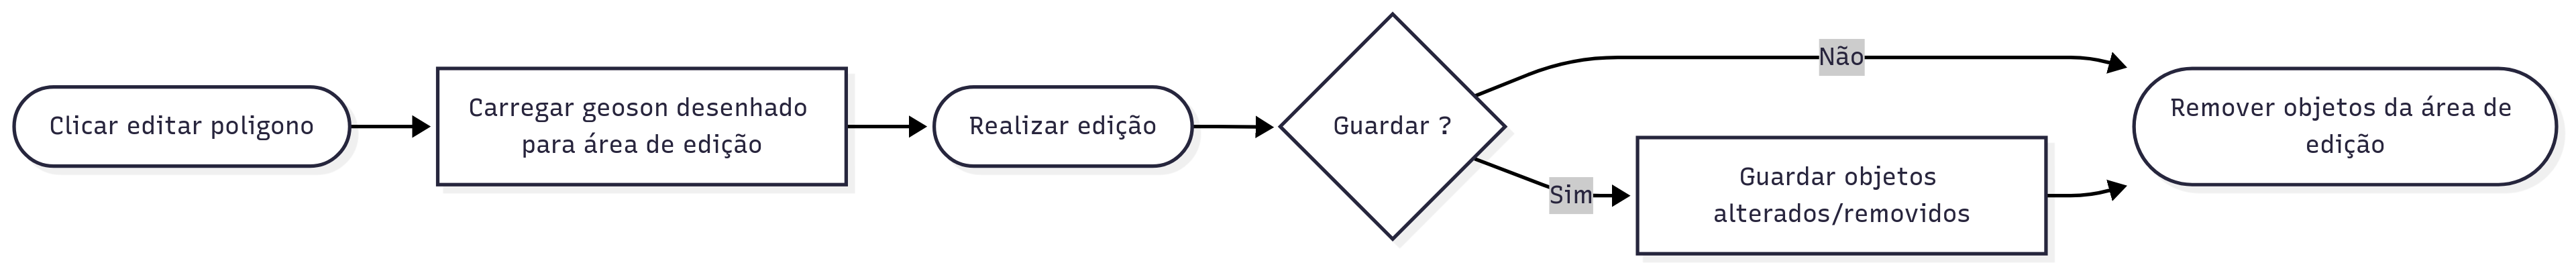
\includegraphics[width=0.85\textwidth]{figs/flowchart_draw.png}
    \caption{\textit{Flow} de edição de poligonos}
    \label{fig:flowchartDraw}
\end{figure}

Após definir o fluxo que pretendia para esta funcionalidade desenvolvi os sistemas responsáveis pele funcionamento do sistema. Da mesma forma que foram criadas \textit{geoJson featuresCollections} para as camadas com pontos, foi também definido uma camada para conter este polígonos.

Ao pressionar o botão de desenhar, altera-se o modo do controlo para desenho. Com este modo ativo, é possível desenhar os polígonos, este modo fica ativado até fechamos o poligono. Ao fechar-se esse polígono, ativa-se um evento, \textit{draw.create}, que obtém a \textit{feature} desenhada, concatena-a com as restantes \textit{features} na camada e desliga o modo de desenho.

Ao pressionar o botão de editar, todas as \textit{features} são carregadas no controlador de desenho e é ativado o modo de edição. Com este modo ativo, o utilizador consegue realizar todo o tipo de alterações, como apagar e redimensionar poligonos. 

Durante o modo de edição, não é permitido ao utilizador criar novos poligonos, esta abordagem foi implementada para evitar a ativação do evento \textit{draw.create}, que poderia causar problemas de integridade na nossa camada. Por fim, ao pressionar o botão de guardar, limpamos a antiga camada e guardamos todos os polígonos, tanto os alterados como os que permanecem inalterados. Ao pressionar no cancelar são simplesmente removidos todos os poligonos do controlador de desenho e o modo de edição é desativado. Existe ainda um botão para remover os poligonos selecionados, que remove simplesmente os que se tem selecionado.

\begin{figure}[!h]
	\centering
	\begin{subfigure}[c]{0.52\textwidth}
		\centering
		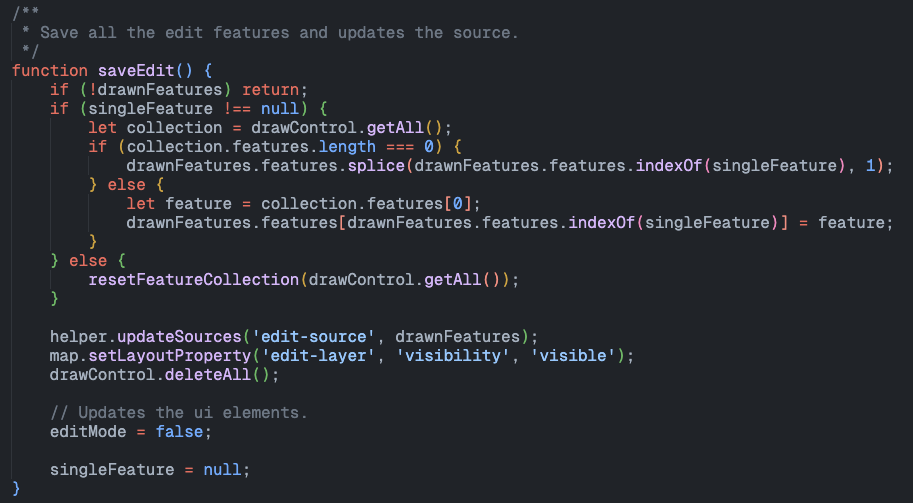
\includegraphics[width=\textwidth]{figs/saveEditFeatures.png}
		\caption{Código guardar \textit{features} editadas}
		\label{fig:saveEditFeature}
	\end{subfigure}
	\hfill
	\begin{subfigure}[c]{0.38\textwidth}
		\centering
		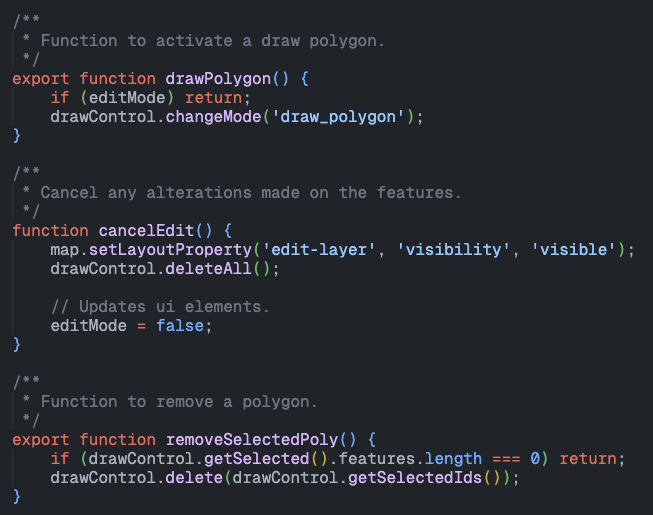
\includegraphics[width=\textwidth]{figs/drawCancelRemove.png}
		\caption{Código desenhar, cancelar e editar}
		\label{fig:drawCancelEdit}
	\end{subfigure}
	\caption{Partes do código de edição de poligonos}
    \label{fig:codeEditPoly}
\end{figure}

% \subsubsection{\textbf{Camada Heatmap}}\label{sec:heatmap}


% \begin{multicols}{2}
% Foi ainda criado, neste componente, uma camada que permite a visualização de um \textit{heatmap}, o qual evidencia os locais com maior concentração de pontos, o que facilita a verificação de padrões nos dados.

% \columnbreak

% \begin{center}
% 	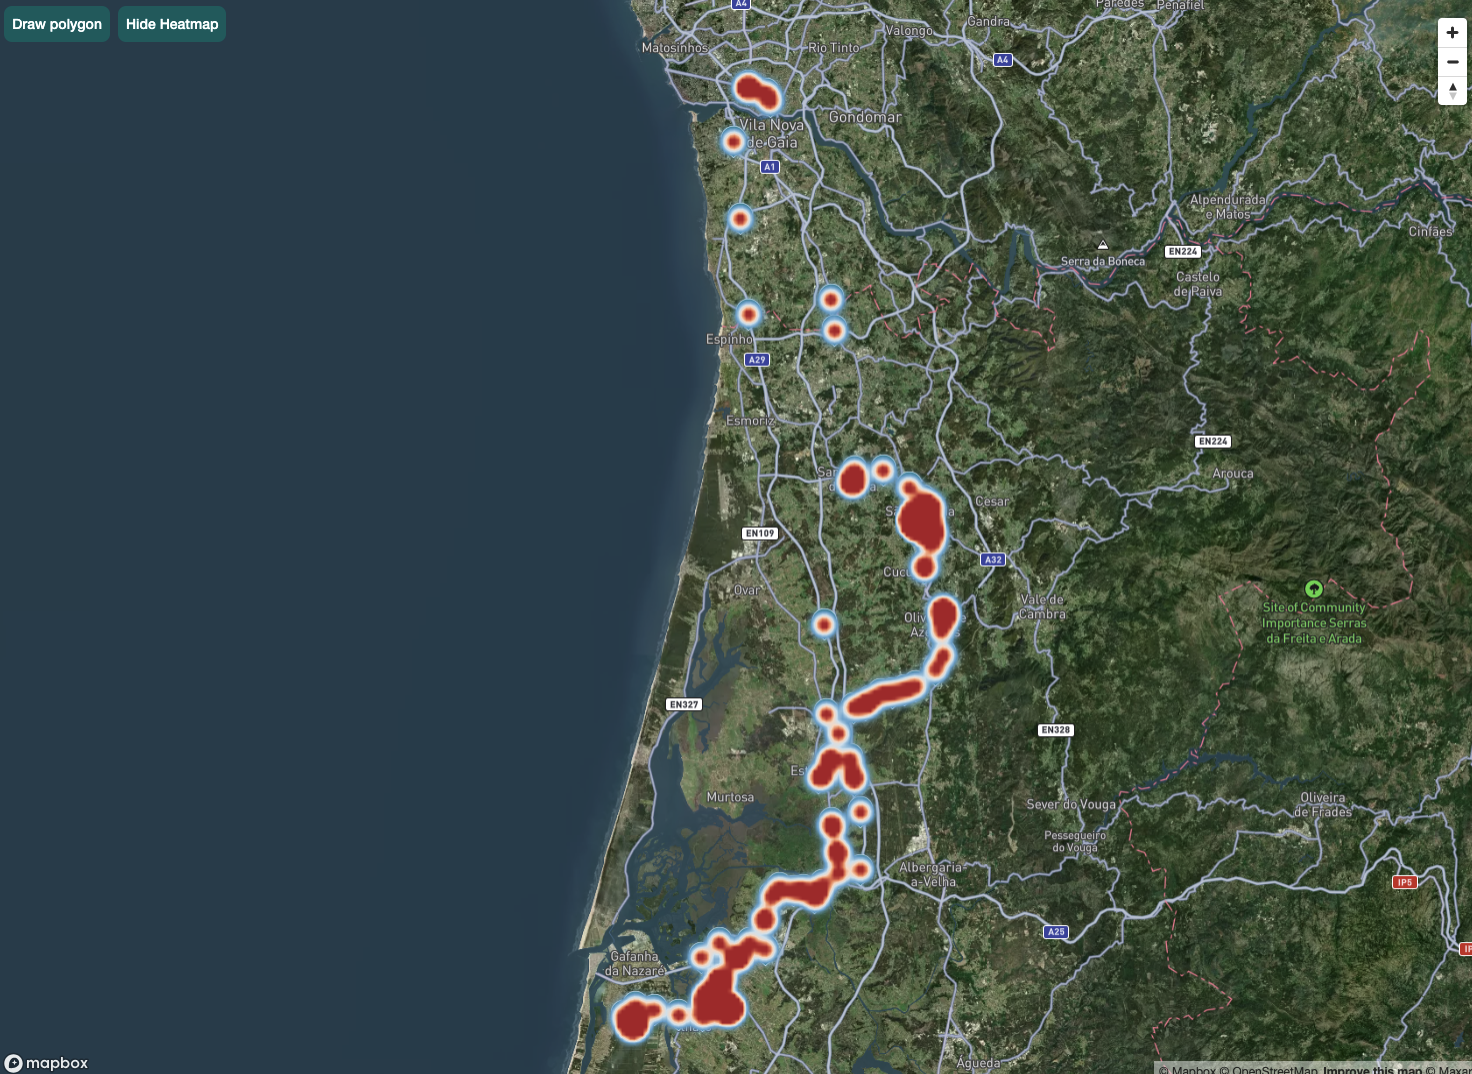
\includegraphics[width=0.8\columnwidth]{figs/heatmap.png}
% 	\captionof{figure}{Camada \textit{heatmap}}
% 	\label{fig:heatmap}
% \end{center}
% \end{multicols}

\clearpage
\subsection{Página \textit{reset palavra-passe}}\label{sec:resetPassword} % Por rever
Uma das tarefas que realizei durante este estágio foi a criação das páginas e do sistema para recuperar palavras-passe. No que diz respeito à interface, foi criada uma nova rota que permite ao utilizador indicar o seu endereço de email para receber um \textit{link} de recuperação, bem como uma página dedicada para a alteração da palavra-passe. 

Todo este sistema foi implementado na mesma rota, \textit{/reset-pass}. Ao aceder a esta página, o utilizador é redirecionados para um ecrã onde lhe é solicitado a inserir o endereço de \textit{email} associado à sua conta. Após inserir o \textit{email} e clicar no botão \textit{"Send password reset email"}, é enviado um \textit{email} com instruções de recuperação. Caso o envio seja bem-sucedido, é apresentada uma mensagem de sucesso ao utilizador.

\begin{figure}[h!]
	\centering
	\begin{subfigure}[c]{0.30\textwidth}
		\centering
		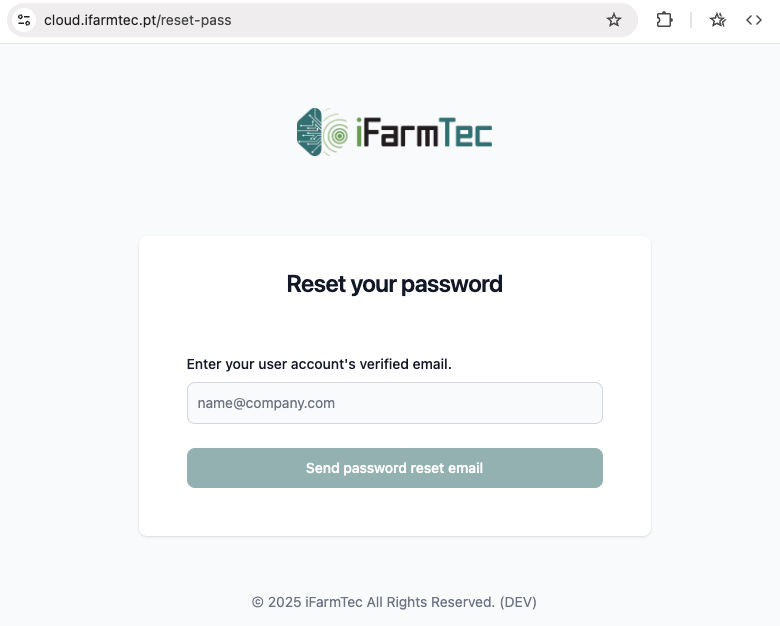
\includegraphics[width=\textwidth]{figs/reset-pass-1.png}
		\caption{\textit{Reset-pass} enviar email}
		\label{fig:resetPassEmail}
	\end{subfigure}
	\hfill
	\begin{subfigure}[c]{0.30\textwidth}
		\centering
		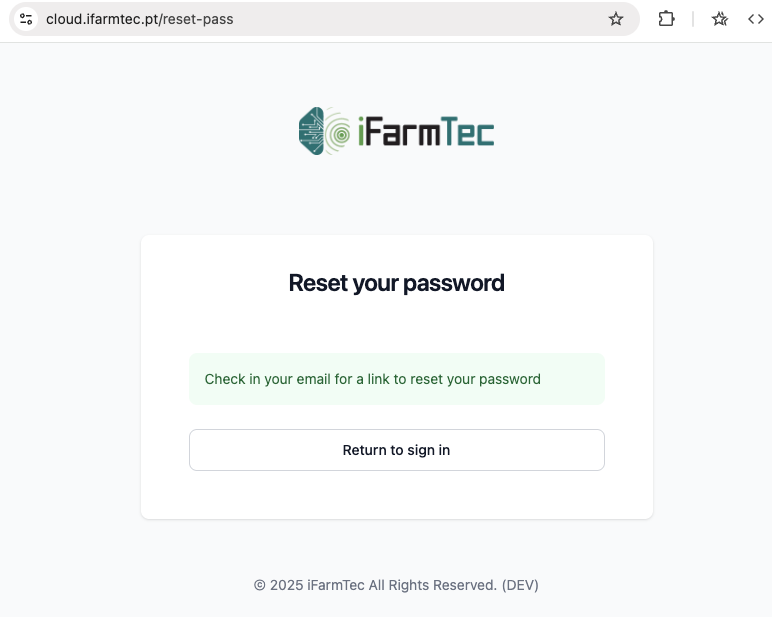
\includegraphics[width=\textwidth]{figs/reset-pass-2.png}
		\caption{\textit{Reset-pass} enviar email, sucesso}
		\label{fig:resetPassEmailSuc}
	\end{subfigure}

		\begin{subfigure}[c]{0.30\textwidth}
		\centering
		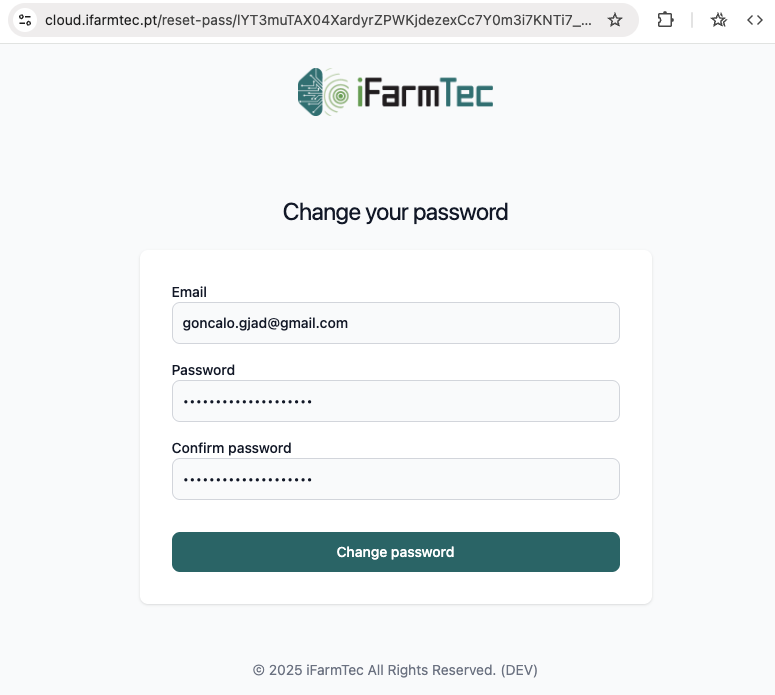
\includegraphics[width=\textwidth]{figs/reset-pass-3.png}
		\caption{\textit{Reset-pass} alterar palavra-passe}
		\label{fig:resetPassReset}
	\end{subfigure}
	\hfill
	\begin{subfigure}[c]{0.30\textwidth}
		\centering
		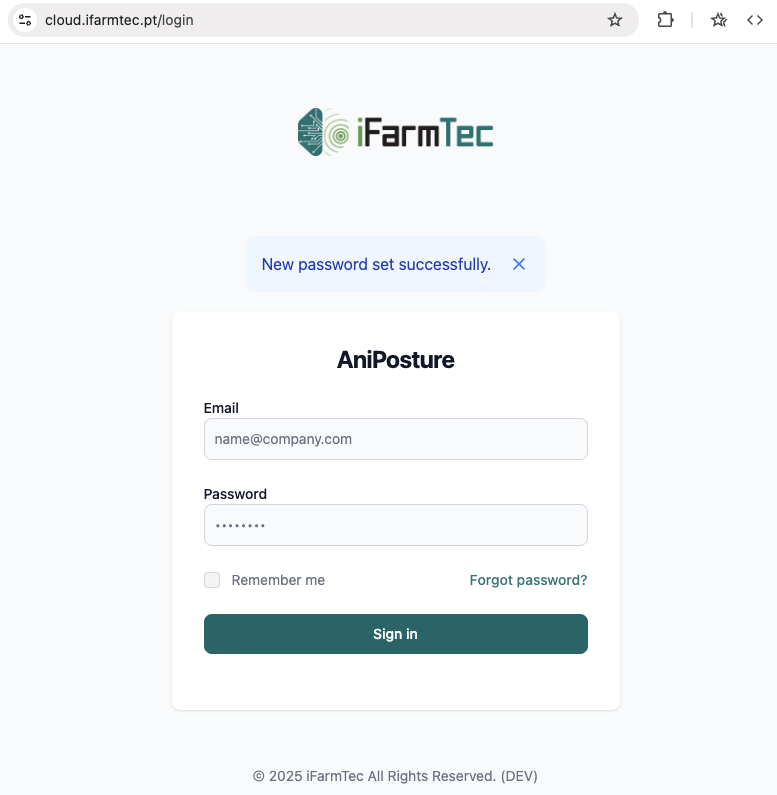
\includegraphics[width=\textwidth]{figs/reset-pass-4.png}
		\caption{Página \textit{login}, palavra-passe alterada}
		\label{fig:resetPassResetSuc}
	\end{subfigure}
	\caption{Páginas \textit{reset-pass}}
    \label{fig:pagResetPass}
\end{figure}

Após a criação desta primeira tela, foi desenvolvida uma segunda página numa sub-rota, \textit{/reset-pass/[token]}. É nesta página que o utilizador pode redefinir a sua palavra-passe. Para tal, deve confirmar o seu endereço de \textit{email} e introduzir a nova palavra-passe.

Foi possível implementar esta funcionalidade graças ao sistema de rotas dinâmicas do \textit{SvelteKit}, ao utilizar o padrão \textit{[slug]}\cite{sveltekit.routing.url}. Este tipo de rota permite criar páginas que recebem parâmetros diretamente na \textit{URL}, o que possibilita o uso da mesma estrutura de rota para diferentes finalidades, basta adicionar o \textit{token} presente no endereço. Após a alteração bem-sucedida da palavra-passe, o utilizador é automaticamente redirecionado para a página de \textit{login}, conforme ilustrado na \autoref{fig:resetPassResetSuc}.

Para tornar todo este sistema funcional e, simultaneamente, garantir que apenas utilizadores autenticados tenham acesso às páginas protegidas, foi implementado um sistema de redirecionamento. Este sistema verifica se o utilizador está autenticado; caso não esteja, é automaticamente redirecionado para a página de \textit{login}. No entanto, existem exceções, nomeadamente as páginas relacionadas com a recuperação de palavra-passe, que permanecem acessíveis mesmo sem autenticação, de forma a permitir que o utilizador consiga redefinir a suas credenciais.

\begin{figure}[h!]
    \centering
    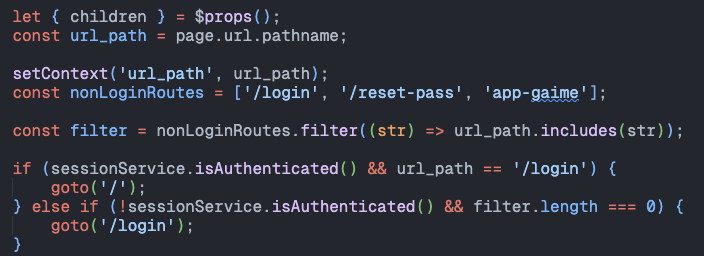
\includegraphics[width=0.6\textwidth]{figs/redirectLogin.png}
    \caption{Redirecionar para o \textit{login}}
    \label{fig:redirectLogin}
\end{figure}

Este código é colocado no ficheiro \textit{layout.svelte} da aplicação, que é responsável por definir uma interface comum a várias páginas. Ao colocá-lo neste ficheiro, garantimos que, sempre que o utilizador tentar aceder a uma página para a qual não tem permissões, ou que não exista, será automaticamente redirecionado para a página de \textit{login} ou para a raiz da aplicação (/).

\subsection{Página de dashboard} % Fechada
Uma das páginas em que mais trabalhei e ajustei ao longo do estágio foi a página do \textit{dashboard}. Nesta página, são apresentadas várias informações relativas aos pacotes enviados por cada dispositivo.


\begin{figure}[!h]
	\centering
	\begin{subfigure}[c]{0.55\textwidth}
        \centering
        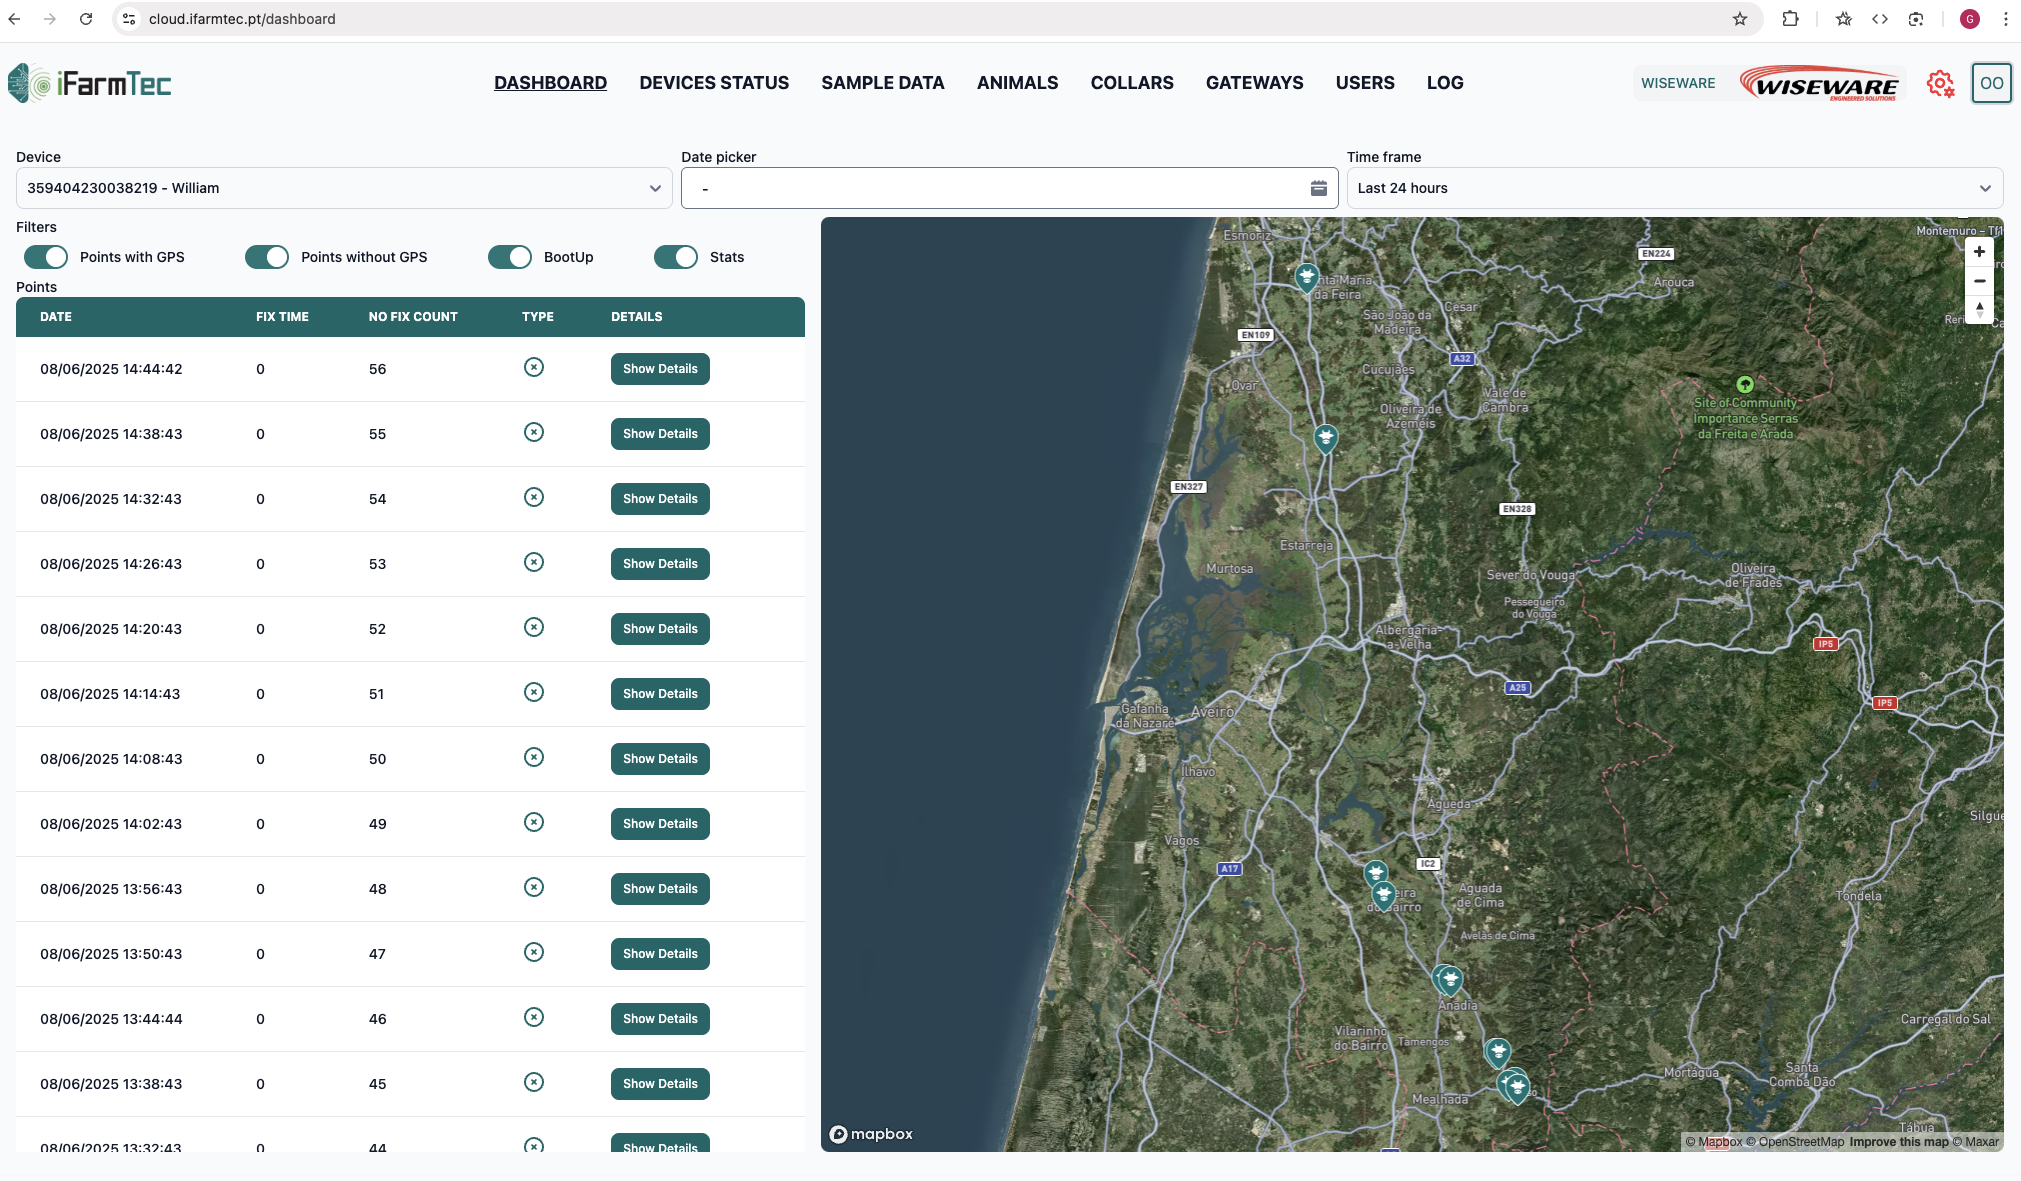
\includegraphics[width=\textwidth]{figs/dashboard.png}
        \caption{Página \textit{dashboard}}
        \label{fig:dashboard}
	\end{subfigure}
	\hfill
	\begin{subfigure}[c]{0.40\textwidth}
        \centering
        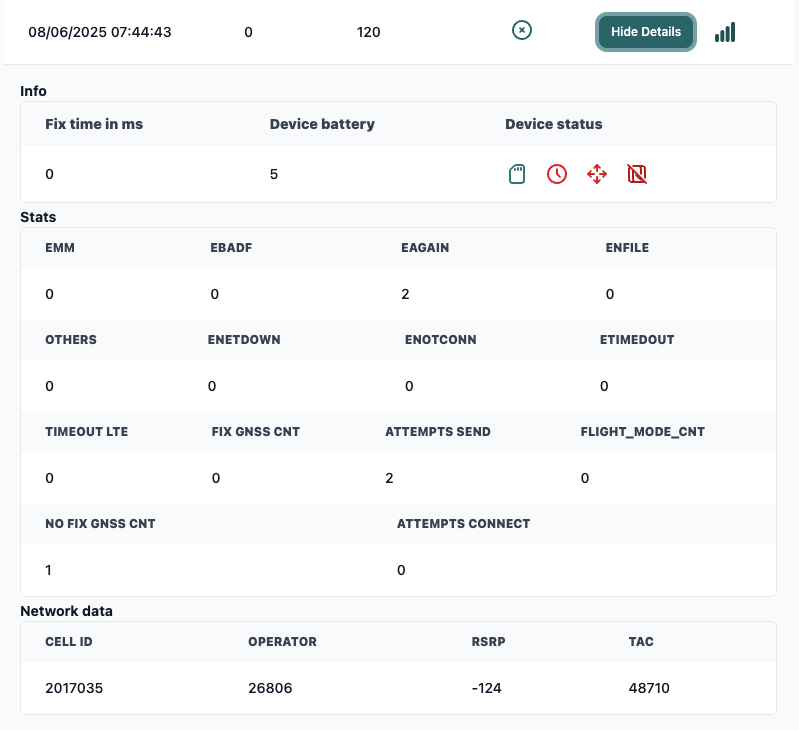
\includegraphics[width=\textwidth]{figs/dashboard-details.png}
        \caption{Detalhes de pacotes}
        \label{fig:packet-details}
	\end{subfigure}
	\caption{Página de \textit{dashboard} e pacotes detalhes}
    \label{fig:dashboard-page}
\end{figure}

Como se pode observar na \autoref{fig:dashboard}, esta página inclui um mapa que representa, através de indicadores, os pontos com coordenadas \acs{gps}. À esquerda do mapa, encontra-se uma lista com todos os pontos registados e, na parte superior da página, estão disponíveis opções para seleção do dispositivo e da data pretendida.

Na \autoref{fig:packet-details}, é possível visualizar o conteúdo apresentado ao clicar no botão de detalhes. Esta secção mostra informações adicionais sobre cada um dos pacotes, incluindo o estado dos periféricos do dispositivo, a data e hora de criação do pacote, dados sobre a rede, entre outros detalhes. Existe também uma secção que permite filtrar os pacotes existentes, o que possibilita ao utilizador visualizar apenas os pacotes com dados \acs{gps}, sem \acs{gps}, pacotes de \textit{boot} ou aqueles que contenham informações adicionais.

\subsection{Página de status}\label{sec:interfaceStatus} % Fechada
Esta página é responsável por apresentar os dispositivos, bem como o uptime diário de cada um deles.

\subsubsection{\textbf{Componente \textit{device stats}}}
Este componente foi desenvolvido com o propósito de mostrar informações sobre cada um dos dispositivos existentes. Para além de dados gerais, como nível da bateria, versão do \textit{hardware}, versão do \textit{firmware}, o número de ficheiros e a data da ultima comunicação, o componente disponibiliza também informação relativa ao \textit{uptime} do dispositivo.

O \textit{uptime} é calculado com base nos pedidos de \acs{gps} realizados pelo dispositivo. Cada dispositivo efetua um pedido de localização a cada 6 minutos, o que resulta num máximo teórico de 240 pedidos por dia. Com base neste valor, é possível determinar a percentagem de tempo em que o dispositivo esteve operacional num determinado dia, \autoref{fig:device-statsComp}.

\begin{figure}[h!]
    \centering
    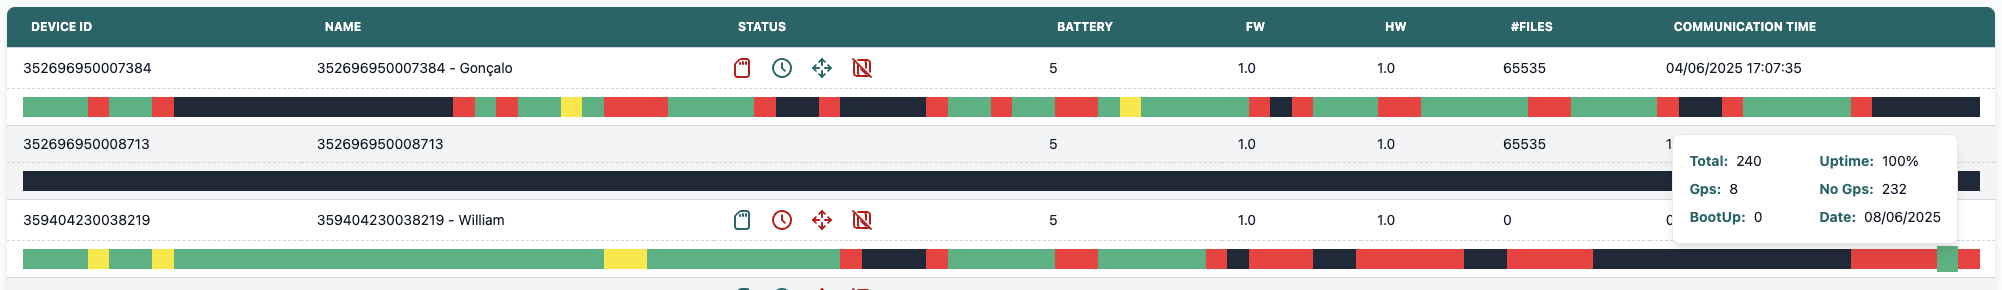
\includegraphics[width=\textwidth]{figs/device-stats.png}
    \caption{Componente \textit{Device stats}}
    \label{fig:device-statsComp}
\end{figure}

\subsubsection{\textbf{Página \textit{device status}}}

Esta página contem, de forma simples, uma tabela composta por múltiplos componentes que apresentam informação relativa a todos os dispositivos registados nesse \textit{tenant}. Como em muitas outras páginas, existe uma caixa de entrada que permite filtrar os dispositivos pelo nome, \autoref{fig:device-statusPage}.

\begin{figure}[h!]
    \centering
    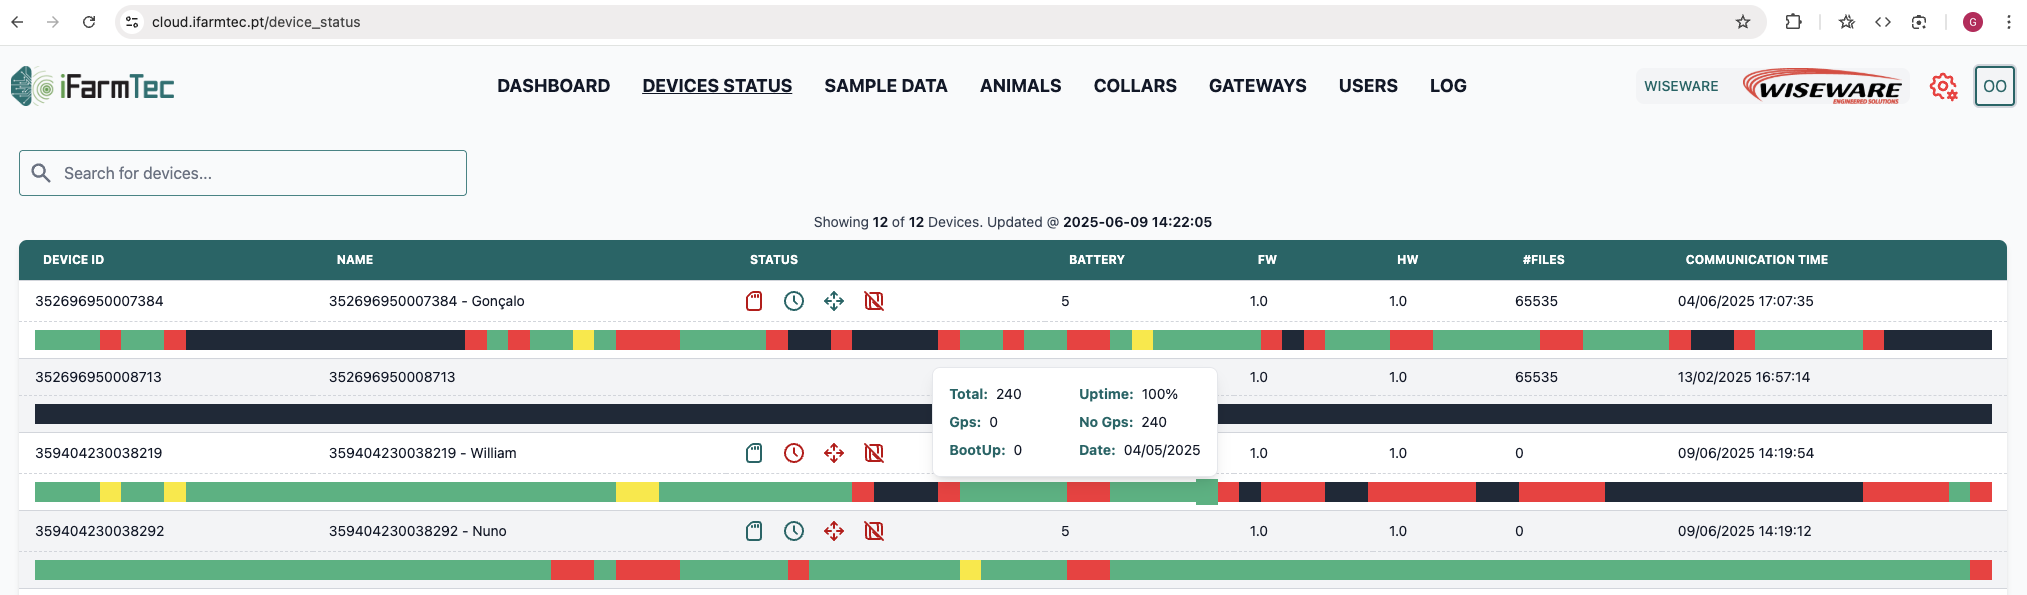
\includegraphics[width=0.95\textwidth]{figs/device_status_page.png}
    \caption{Página \textit{device status}}
    \label{fig:device-statusPage}
\end{figure}

\subsection{Página de utilizadores} 
A página foi criada a partir de outra já existente na aplicação. Anteriormente, existia uma página exclusiva para os \textit{Owners} do projeto, onde era possível remover e adicionar utilizadores aos \textit{tenants}, desativá-los, promovê-los a administradores de cada \textit{tenant} e enviar um email para recuperação da palavra-passe. Foram efetuadas alterações nessa página com o intuito de manter um design mais consistente.

A nova página destina-se exclusivamente aos administradores dos \textit{tenants}. Nela, os administradores podem adicionar novos utilizadores ao \textit{tenant}, desativá-lo, promovê-lo a administrador e enviar emails para recuperação da palavra-passe.

\begin{figure}[!h]
	\centering
	\begin{subfigure}[c]{0.45\textwidth}
		\centering
		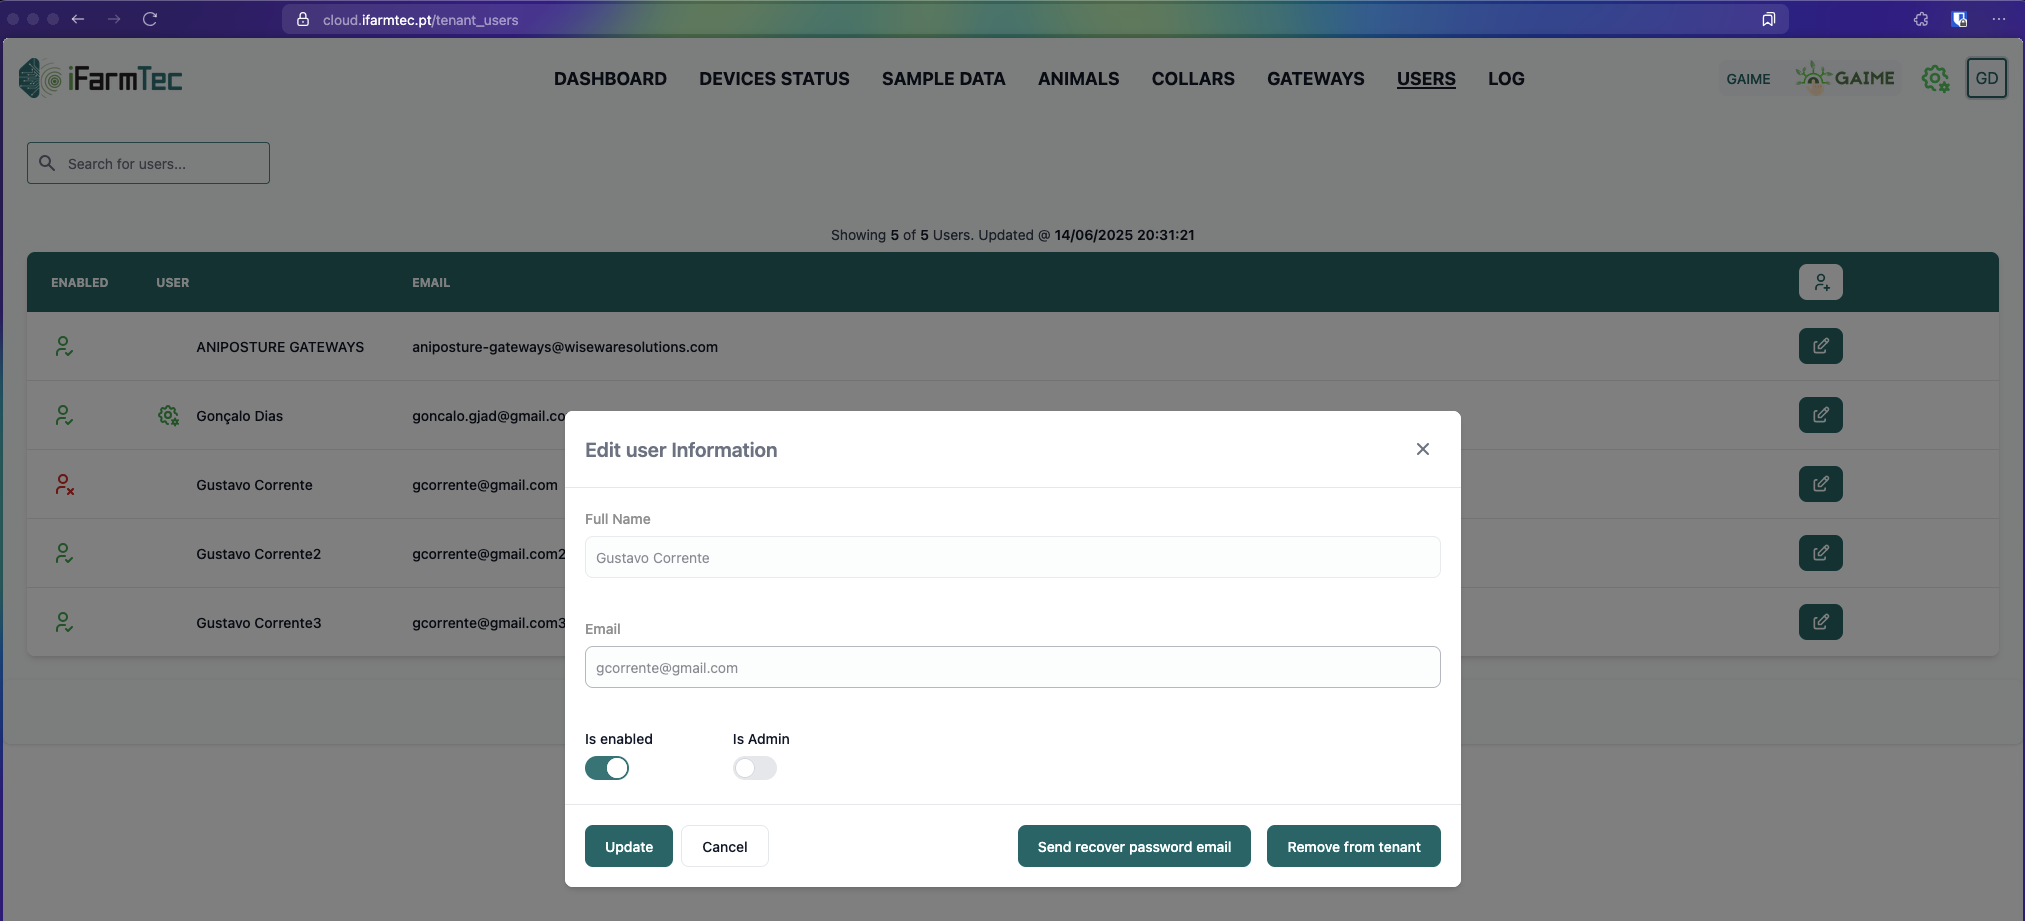
\includegraphics[width=\textwidth]{figs/userAdmin.png}
		\caption{Página \textit{user} para \textit{tenant admins}}
		\label{fig:user-Admin}
	\end{subfigure}
	\hfill
	\begin{subfigure}[c]{0.45\textwidth}
		\centering
		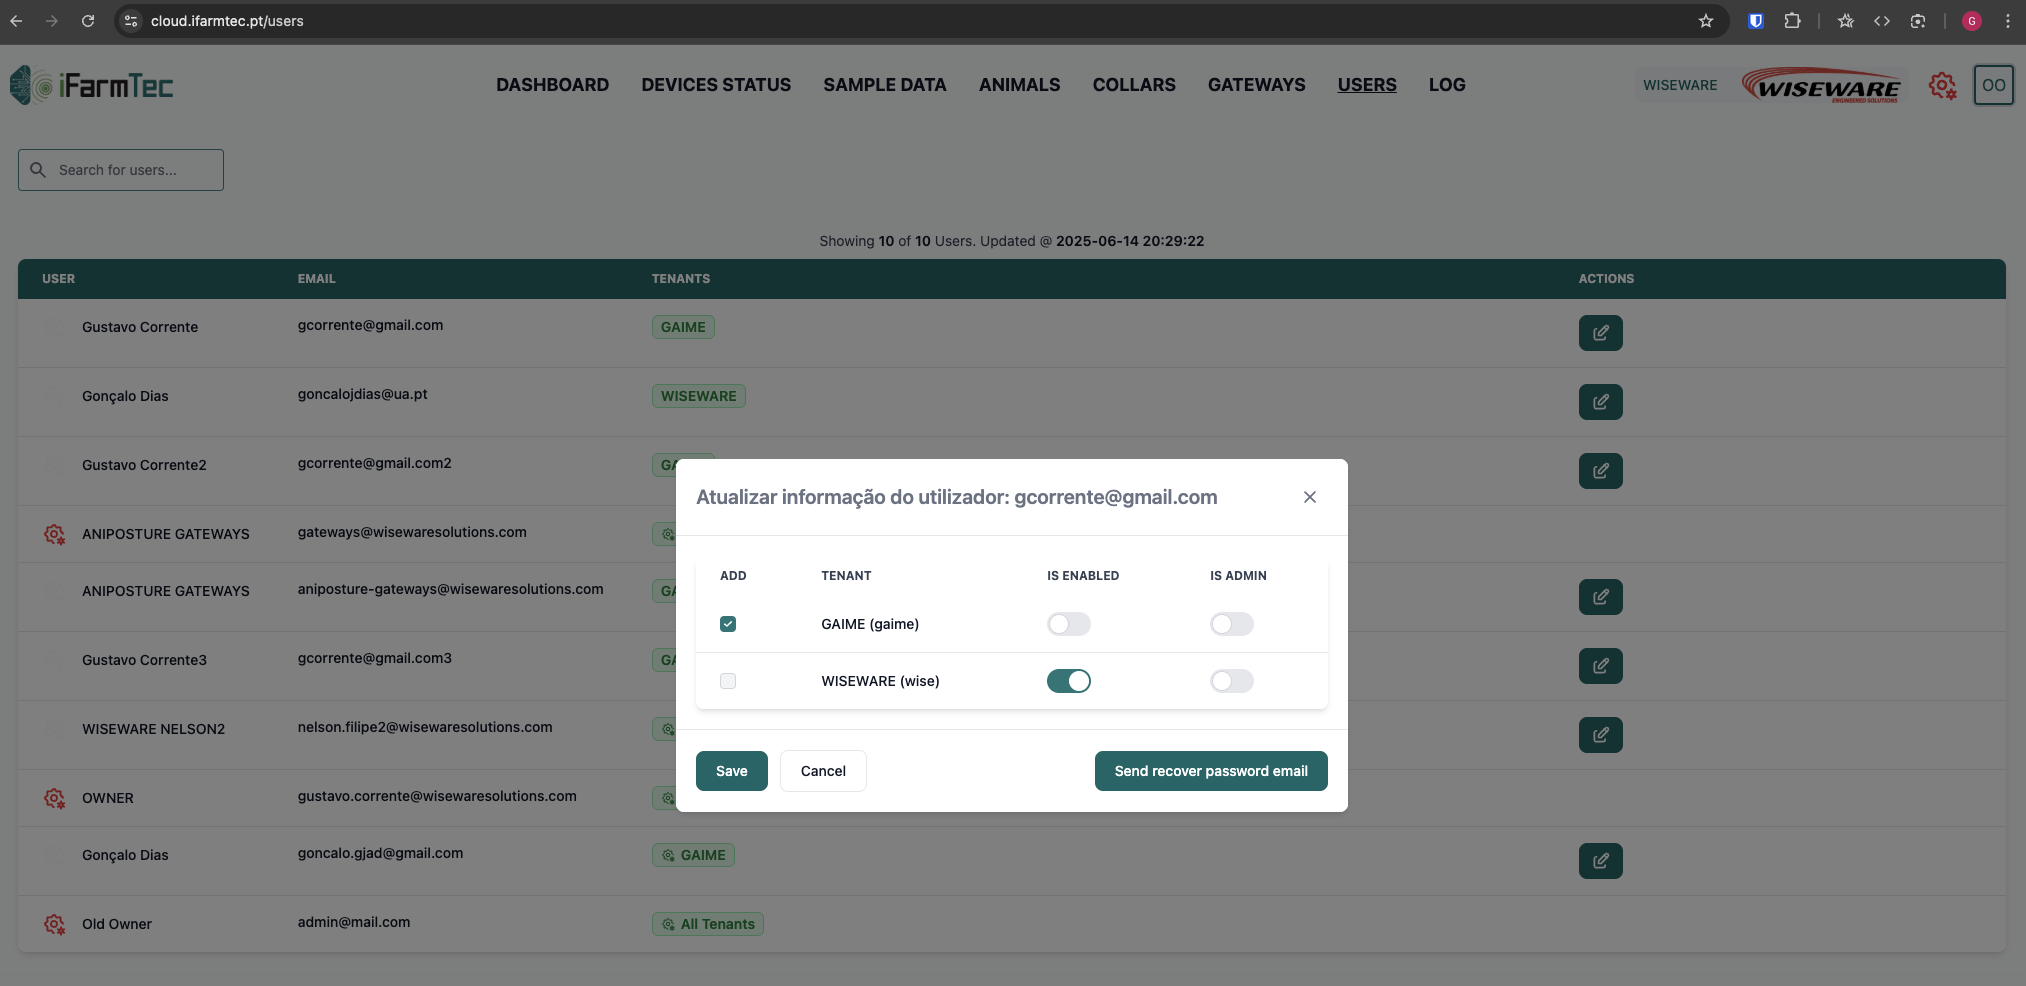
\includegraphics[width=\textwidth]{figs/userOWNER.png}
		\caption{Página \textit{user} para \textit{owners}}
		\label{fig:user-Owner}
	\end{subfigure}
	\caption{Páginas para gerir utilizadores}
    \label{fig:gestUsers}
\end{figure}

Nesta fase de desenvolvimento, procedi a uma pequena alteração na \textit{nav bar} para que esta torne-se dinâmica, adapte-se às permissões dos utilizadores. Assim, os utilizadores normais não têm acesso ao link para gestão de utilizadores, os administradores são redirecionados para \textit{/tenant\_users} e os \textit{owners} para \textit{/users}.

\clearpage
\subsection{Página de gráficos} % Fechada

Nesta secção é apresentado um gráfico com os dados do acelerómetro e da temperatura do dispositivo, ao longo de um determinado intervalo de tempo. 

\subsubsection{\textbf{Componente \textit{Echarts}}}
Foi desenvolvido um componente para o motor gráfico escolhido, \autoref{sec:echarts}, pela sua flexibilidade e capacidade de visualização interativa. Este componente foi concebido de forma reutilizável, o que permite representar diferentes tipos de dados provenientes dos sensores, ao utilizar gráficos distintos, como linhas ou barras, conforme a necessidade.   

O componente foi desenhado com o foco no desempenho e facilidade de utilização, o que garante assim uma boa experiencia, tanto para o utilizador final como para o programador. O gráfico também permite a atualização dinâmica dos dados e a interação com o utilizador através de funcionalidades como zoom e seleção de intervalos.

Os dados provenientes do acelarômetro são apresentados de forma normalizada, ao utilizar a seguinte formula:
\begin{math}
	\sqrt{x^2 + y^2 + z^2}
\end{math}
.

Esta normalização permite obter um valor que representa a intensidade de movimento do animal, o que facilita uma análise visual mais clara e concisa. Simultaneamente, a variação da temperatura é apresentada no mesmo gráfico, mas num eixo distinto, o que possibilita a correlação entre a temperatura e o movimento do animal.

Surgiu um contratempo durante a realização desta página. Para apresentar os dados de forma mais fidedigna, de modo a perceber o \textit{uptime} e \textit{downtime} dos dispositivos, foi necessário mostrar, propositadamente, lacunas nos dados. Para tal, foi necessário criar uma lista com todas os minutos existentes durante o período de pesquisa, o que gera 1440 registos para um único dia, 24 horas. Posteriormente, verificava-se se cada uma das amostras pertencia a um determinado minuto. Se pertencia, apresentavam-se os valores do acelerómetro e da temperatura com a data, hora, minuto e segundo da sua recolha. Caso contrário, inseria-se um valor nulo, de modo a assinalar a ausência de amostra nesse momento.
% \begin{wrapfigure}{r}{0.5\textwidth}
%   \begin{center}
%     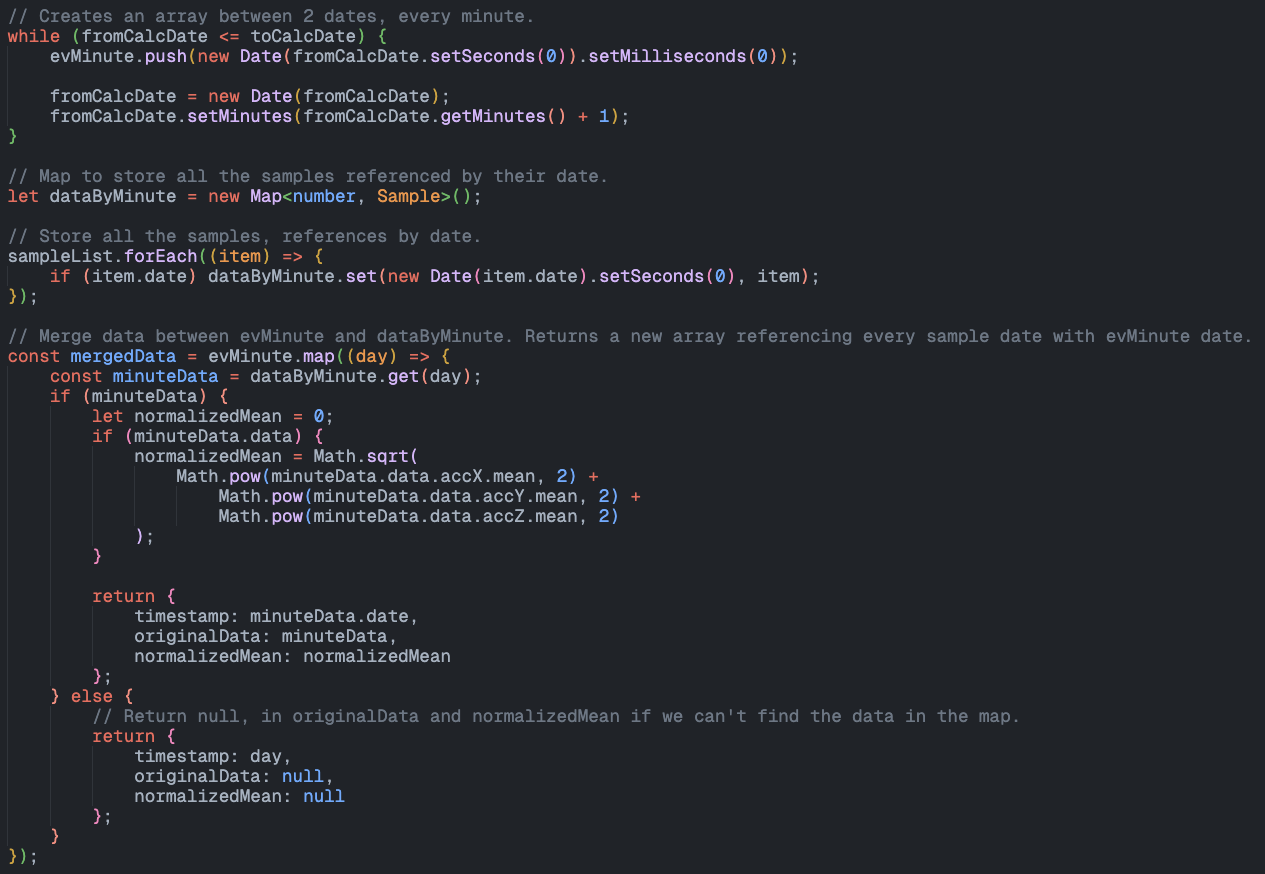
\includegraphics[width=0.48\textwidth]{figs/echartData.png}
%   \end{center}
%   \caption{Codigo verificar acelarômetro e temperatura}
%   \label{fig:selectAccAndTemp}
% \end{wrapfigure}

\begin{figure}[!h]
	\centering
	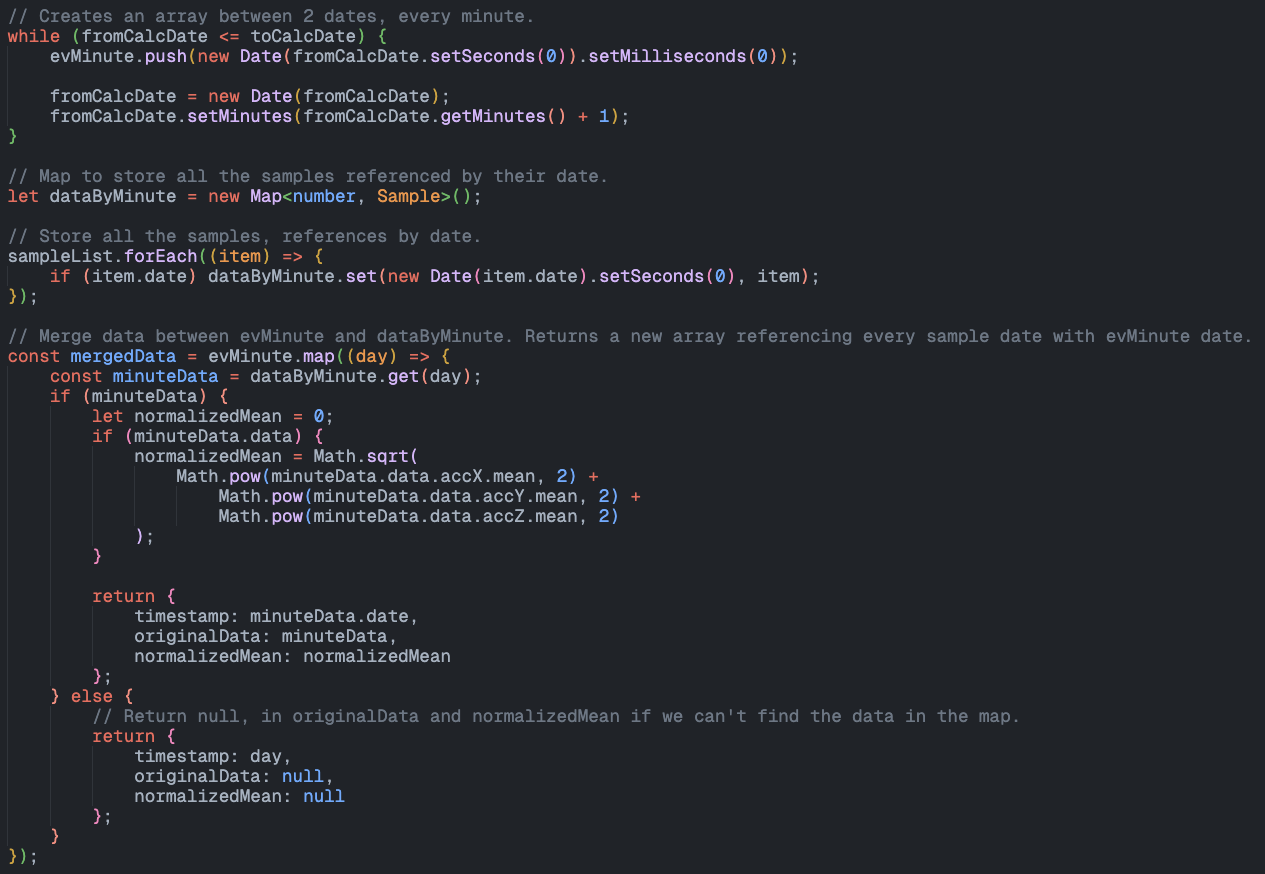
\includegraphics[width=0.47\textwidth]{figs/echartData.png}
	\caption{Codigo verificar acelarômetro e temperatura}
	\label{fig:selectAccAndTemp}
\end{figure}

\clearpage
\subsection{Página de erro} % Fechada
Foi criada uma nova página de erro, mais alinhada com o design da aplicação. Para a sua implementação, conforme ilustrado na \autoref{fig:404}, foi utilizada uma funcionalidade nativa do \textit{sveltekit}. Ao criar uma página de erro na raiz da aplicação, como demonstrado na \autoref{fig:errorRoute}, todos os erros que ocorram durante a navegação são automaticamente redirecionados para essa página.

Desta forma, foi possível desenvolver uma página de erro genérica, aplicável a qualquer secção da aplicação, cuja apresentação adapta-se dinamicamente consoante o tipo de erro ocorrido.

\begin{figure}[!h]
	\centering
	\begin{subfigure}[c]{0.80\textwidth}
		\centering
		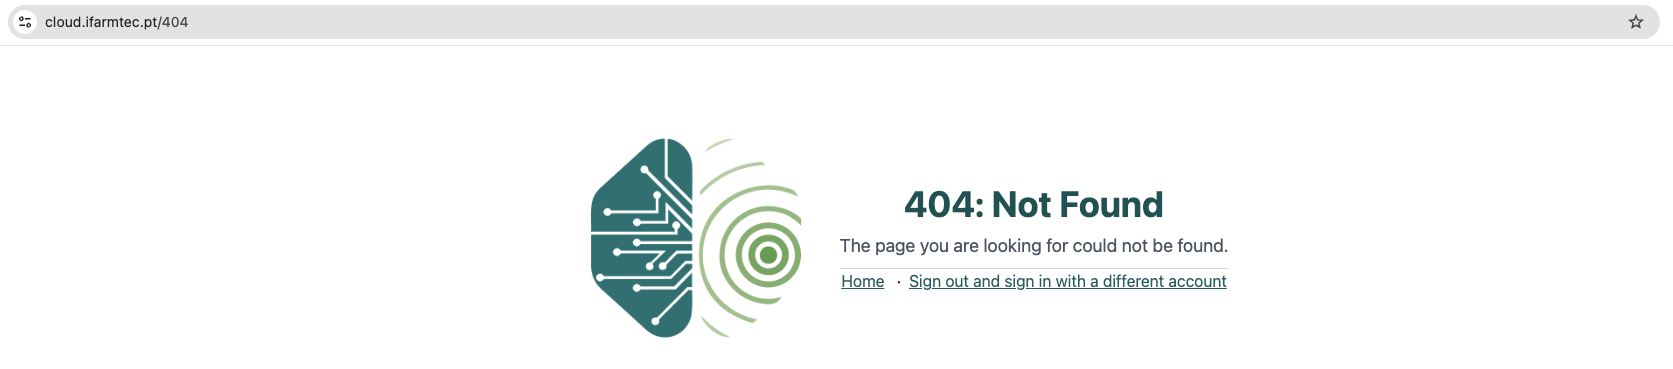
\includegraphics[width=\textwidth]{figs/404.png}
		\caption{Página de erro}
		\label{fig:404}
	\end{subfigure}
	\hfill
	\begin{subfigure}[c]{0.15\textwidth}
        \centering
        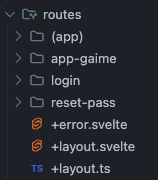
\includegraphics[width=\textwidth]{figs/errorRoute.png}
        \caption{\textit{error.svelte}}
        \label{fig:errorRoute}
	\end{subfigure}
	\caption{Erro}
\end{figure}

\subsection{Componente data hora} % Fechada
A biblioteca de componentes, \textit{flowbite}, não contém nenhum componente que permita ao utilizador selecionar uma data e hora para cada dia. Decidi então desenvolver um componente próprio. Para tal, reutilizei o componente de seleção de data do \textit{flowbite} e adicionei um campo que permite a seleção das horas. Neste caso, o primeiro campo de hora corresponde ao primeiro dia, e o segundo ao segundo dia. Assim, conseguimos selecionar de forma mais precisa os intervalos desejados para a pesquisa.

\begin{figure}[!h]
	\centering
	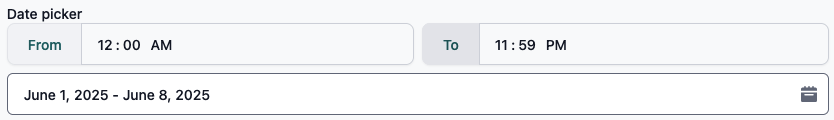
\includegraphics[width=\textwidth]{figs/datepicker.png}
	\caption{Componente \textit{Datepicker}}
	\label{fig:Datepicker}
\end{figure}

\begin{multicols}{2}
Tive ainda de criar algumas funcionalidades no componente para definir automaticamente as horas e as datas ao seleciona-las.

\columnbreak

\begin{center}
	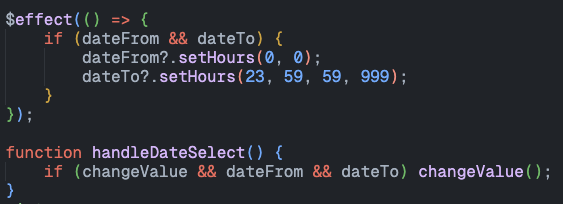
\includegraphics[width=0.8\columnwidth]{figs/componenteClick.png}
	\captionof{figure}{Selecionar data no componente \textit{Datepicker}}
	\label{fig:SelecionarDatepicker}
\end{center}
\end{multicols}

\clearpage
\subsection{Rotas sem inicio de sessão}\label{sec:noLoginInterface} % Fechada
Uma das últimas tarefas que foram-me atribuídas durante o estágio foi a criação de duas rotas que permitissem a visualização de dados dos dispositivos sem necessidade de autenticação. A nova rota foi chamada de \textit{/app-gaime} e inclui duas sub-rotas: \textit{/map} e \textit{/chart}.

\begin{multicols}{2}
	\begin{center}
        \centering
		\includegraphics[width=0.8\columnwidth]{figs/appGaimeMap.png}
		\captionof{figure}{Página \textit{app-gaime/map}}
		\label{fig:appGaimeMap}
	\end{center}

\columnbreak

\begin{center}
		\centering
        \includegraphics[width=0.8\columnwidth]{figs/appGaimeChart.png}
		\captionof{figure}{Página \textit{app-gaime/chart}}
        \label{fig:appGaimeChart}
\end{center}
\end{multicols}

Para selecionar o dispositivo do qual queremos ver os dados, é necessário introduzir o seu \textit{id} na barra de pesquisa, \textit{/app-gaime/[device\_id]}.

Por padrão, a rota do mapa , \autoref{fig:appGaimeMap}, solicita ao servidor todos os pontos com coordenadas \acs{gps} registados nas últimas 24 horas. De forma semelhante, a rota do gráfico, \autoref{fig:appGaimeChart}, recupera informações relativas ao acelarômetro e temperatura no mesmo intervalo de tempo. 

A quantidade de horas solicitadas ao servidor podem ser alteradas através de um \textit{query param}, ao utilizar o formato \textit{?h=[número de horas]}.

\subsection{Guardar filtros}\label{sec:saveFilters} % Fechada
Para melhorar a usabilidade da aplicação, foram implementadas funcionalidades que tornam permanentes os filtros selecionados pelo utilizador. Dessa forma, ao mudar de página ou fechar a aplicação, as opções permanecem previamente selecionadas. Esta funcionalidade foi construída com base numa biblioteca existente, conforme descrito em \citetitle{persisted-store.joshnuss.url} \cite{persisted-store.joshnuss.url}.

A referida biblioteca simplifica a utilização das \textit{stores} do \textit{Svelte}, armazena informações no \textit{local storage} do \textit{browser}. Essa abordagem permite ao utilizador navegar entre as páginas sem perder os filtros previamente definidos.


\begin{multicols}{2}
	\begin{center}
        \centering
        \includegraphics[width=0.9\columnwidth]{figs/store.svelte.png}
		\captionof{figure}{Utilização das \textit{stores} num ficheiro \textit{.svelte}}
        \label{fig:store.svelte}
	\end{center}

\columnbreak

\begin{center}
		\centering
		\includegraphics[width=0.9\columnwidth]{figs/store.png}
		\captionof{figure}{Criação das \textit{stores}}
		\label{fig:store}
\end{center}
\end{multicols}

\clearpage
\section{Servidor da aplicação}
Este projeto utiliza um servidor desenvolvido em \textit{Java}, responsável por armazenar os dados enviados pelos dispositivos, criar e autenticar utilizadores, assim como obter informações através de diferentes rotas, entre outras funcionalidades.

\subsection{O que é o \textit{backend} ?}
Como mencionado anteriormente, o \textit{backend} é desenvolvido em \textit{Java} e adota uma arquitetura do tipo \textit{Controller-Service-Repository}. Esta abordagem divide a aplicação em três camadas: os \textit{Controllers} gerem as requisições e respostas, os \textit{Services} implementam a lógica de negócio e os \textit{Repositories} cuidam do acesso à base de dados. Para implementar esta arquitetura de forma mais eficiente e com melhor desempenho, foram utilizadas diversas bibliotecas de apoio.

\subsubsection{\textbf{Vert.x}}
O \textit{Vert.x} é uma \textit{biblioteca} assincrona e reativa para o \acs{jvm}, utilizada no desenvolvimento de aplicações concorrentes, escaláveis e de elevado desempenho, como \textit{\acs{api}s} e sistemas baseados em eventos. No nosso caso o \textit{Vert.x} é utilizado para desenvolver a \acs{api} do projeto, definir rotas, criar serviços, enviar \textit{email}, entre outras funcionalidades.

\subsubsection{\textbf{Ebean \acs{orm}}}
A componente do \textit{Repository} (repositório) é desenvolvida com o auxílio do \textit{Ebean \acs{orm}}. Esta \textit{framework} suporta múltiplos níveis de abstração de consultas, incluindo consultas \acs{orm}, consultas \acs{sql}, entre outros. O \textit{Ebean} é compatível com diversos sistemas de bases de dados, como \textit{Postgres} e \textit{MySQL}. Além disso, utiliza anotações de mapeamento \acs{jpa} e disponibiliza mapeamentos adicionais, como \textit{@DBJson} e \textit{@DBArray}.

\subsubsection{\textbf{Postgres}}
O \textit{Postgres} é o sistema de base de dados utilizado neste projeto. Não só permite a utilização de pontos \acs{gps}, como destaca-se pela sua rapidez, escalabilidade e robustez. Adicionalmente, garante a alta disponibilidade e integridade dos dados, esta capacidade promove a execução de consultas complexas e a implementação de estratégias de replicação, o que assegura a continuidade do serviço mesmo em ambientes de elevada concorrência e carga.

\subsubsection{\textbf{Funcionamento do projeto}}
Neste caso, o projeto funciona da seguinte forma. Existem dois "projetos" dentro do mesmo sistema, ou seja, há um projeto base que contém o conjunto de funcionalidades comuns a outros projetos, incluindo a autenticação de utilizadores, o sistema de \textit{tenants}, o envio de \textit{emails}, entre outros.

Dentro deste projeto base, encontra-se um sub-projeto específico, no nosso caso referido por \textit{aniposture}, que reúne as ações específicas, tais como a gestão de dispositivos, gateways, animais, o servidor \textit{UDP} para receção pacotes \acs{gps}, entre outros.

\subsection{Rota para obter número de pedidos por dispositivo} % REVER
% Este foi dos trabalhos mais interessantes que realizei, simples mas muito  interessante. Foi "desafiado" a alterar uma das rotas da aplicação de forma a deixa-la mais util e com mais informação. 

% A rota que já existia mostrava a quantidade de pedidos realizados por cada dispositivo, podiamos inserir as datas, de quanto até quando queriamos os dados e o dispositivo a pesquisar. Ela retornava os os dados de cada dispositivo por dia, tinha apenas um senão, os dados do dia atual só eram mostrados no dia seguinte. 

% Apesar de cumprir o seu serviço inicial, mostrar como os dispositivos estavam a comunicar, tinha pontos negativo, apenas poder ver os dados no dia seguinte, termos de ser especificos numa data, entre outras.

% Para a tornar melhor fiz as seguintes alterações, para cada pedidos apenas enviamos dois dados, o dispositivo e a quantidade de dias que queremos pesquisar. A rota vai retornar dados detalhados, como a quantidade de pontos \acs{gps}, pontos sem \acs{gps} e os pontos de \textit{boot}, pontos que são enviados quando o dispositivo liga-se à rede, e também o total de pontos por dia. Com isto também envia os dias onde não existiu comunicação, desta forma conseguimos ver se o dispositivo naquele dia teve algum problema.

Este foi um dos trabalhos mais interessantes que realizei. Fui "desafiado" a alterar uma das rotas da aplicação para a tornar mais útil e com mais informação.

A rota preexistente exibia a quantidade de pedidos efetuados por cada dispositivo. Permitia inserir as datas, desde e até quando, e o dispositivo a pesquisar. Retornava os dados de cada dispositivo por dia, mas apresentava um senão: os dados do dia atual apenas estavam disponíveis no dia seguinte.

Apesar de cumprir a sua função inicial, que era mostrar como os dispositivos comunicavam, a rota tinha pontos negativos, tais como a consulta dos dados ser apenas possível no dia seguinte ou a necessidade de especificar uma data, entre outros.

Para a melhorar, realizei as seguintes alterações: para cada pedido, enviam-se agora apenas dois dados, o dispositivo e a quantidade de dias a pesquisar. A rota passa a retornar dados detalhados, como a quantidade de pontos \acs{gps}, de pontos sem \acs{gps} e os registos de \textit{boot}, que são enviados quando o dispositivo liga-se à rede, e também o total de pontos por dia. Com estas alterações, são também reportados os dias em que não houve comunicação. Desta forma, é possível identificar se o dispositivo apresentou alguma anomalia nesse dia.

% \subsubsection{\textbf{SQL}}
% Para realizar esta rota, um pouco mais complexa do que outras, utilizei \acs{sql} puro em vez da \acs{orm}. As \acs{orm} são muito interessantes quando temos rotas mais simples, mas neste caso provavelmente seria um problema.

% Esta \textit{query} conta com o seguinte, duas relações temporárias, uma para obter os todos os dias selecionados naquele \textit{time frame} e outra para obter o dados do dispositivo. Depois é feita uma \textit{query}, às duas tabelas temporárias, onde fazemos a relação entre cada dia, da tabela de dias e da tabela de pontos. Fazemos o filtro por cada tipo de ponto e a soma de todos eles de forma a obtermos os dados necessários. 

% Se tivermos no dia atual é feita uma pesquisa a todos os pontos realizados até às zero horas do dia.

% Esta rota foi com o propósito de alimentar uma das páginas da a interface do projeto, a rota antiga, mostrava informações apenas sobre os pontos, já esta mostra informações sobre os dias e os pontos realizados em cada dia.


\begin{figure}[!h]
	\centering
	\begin{subfigure}[c]{0.45\textwidth}
		\centering
		\includegraphics[width=\textwidth]{figs/sqlCountDaily.png}
		\caption{SQL para rota \textit{/countDaily}, antiga rota.}
		\label{fig:sqlCountDaily}
	\end{subfigure}
	\hfill
	\begin{subfigure}[c]{0.45\textwidth}
        \centering
        \includegraphics[width=\textwidth]{figs/return_old_query.png}
		\caption{Resultado da \textit{query} antiga}
        \label{fig:returnOldQuery}
	\end{subfigure}
	\caption{Antiga \textit{query} para obter o estado dos dispositivos}
\end{figure}


\subsubsection{\textbf{SQL}}
Para concretizar esta rota, algo mais complexa que outras, optei por utilizar \acs{sql} puro em vez da \acs{orm}. As \acs{orm} são bastante úteis para rotas mais simples, mas, neste caso, o seu uso representaria provavelmente um problema.

Esta \textit{query} integra o seguinte: duas relações temporárias, uma para obter todos os dias selecionados no período definido e outra para recolher os dados do dispositivo. Posteriormente, é efetuada uma \textit{query} sobre as duas tabelas temporárias, estabelecendo a relação entre cada dia, da tabela de dias, e os pontos da tabela de pontos. Realiza-se a filtragem por cada tipo de ponto e a soma de todos eles, de modo a obter os dados necessários.

\begin{figure}[!h]
	\centering
	\begin{subfigure}[c]{0.45\textwidth}
		\centering
		\includegraphics[width=\textwidth]{figs/sqlCountFrame.png}
		\caption{SQL para rota \textit{/countFrame}, nova rota.}
		\label{fig:sqlCountFrame}
	\end{subfigure}
	\hfill
	\begin{subfigure}[c]{0.45\textwidth}
        \centering
        \includegraphics[width=\textwidth]{figs/return_new_query.png}
		\caption{Resultado da nova \textit{query}}
        \label{fig:returnNewQuery}
	\end{subfigure}
	\caption{Nova \textit{query} para obter o estado dos dispositivos}
\end{figure}


No caso do dia atual, efetua-se uma pesquisa de todos os pontos registados até às zero horas desse dia.

Esta rota teve como propósito alimentar uma das páginas da interface do projeto, \autoref{sec:interfaceStatus}. Enquanto a rota anterior mostrava apenas informações sobre os pontos, esta exibe dados detalhados sobre os dias e os pontos registados em cada um.

Esta reestruturação não só otimizou a rota em termos de dados, mas também conferiu um valor analítico superior. A capacidade de identificar dias sem comunicação, permite diagnosticar falhas de conexão ou potenciais anomalias nos dispositivos, algo que a versão anterior não proporcionava.

A opção por \acs{sql} em detrimento da \acs{orm} revelou-se essencial para assegurar a agregação complexa de diversos tipos de pontos, com \acs{gps}, sem \acs{gps} e de \textit{boot}. A deteção de períodos sem atividade fornece à interface dados mais robustos e detalhados para o utilizador.

\clearpage
\subsection{Sistema de envio de emails} % REVER
% O sistema de emails foi outra das alterações que realizei durante o estágio. Dentro do proprio \textit{backend} já existia a configuração de email a funcionar, mas existiam alguns pontos que faziam o envio não funcionar.

% Foram corrigidos alguns problemas, nas rotas de \textit{reset-pass} e \textit{change-pass}, a \textit{reset-pass} é responsável por enviar o email para o utilizador. Foram feitas aqui alterações, principalmente no \textit{template} do email. O template que existia não fazia sentido com o \textit{design system} da aplicação, nem com o seu propósito.

% Já a outra rota \textit{change-pass} é onde é então realizada a alteração da \textit{password}. Aqui foi encontrado um problema, podemos dizer, incomum. Ao criarmos o \textit{hash} da nova password, era chamada a função de \textit{hash} no \textit{controller} e \textit{service}, ao fazer isto era criado o \textit{hash} da \textit{hash}. Desta forma era impossível fazer login com a password definida.

% Foram também realizadas outras mudanças nesta rota, verificação do \textit{token}, alteração do seu formato, conter apenas letras minúsculas, maiúsculas, traços e \textit{underscores}. Não contém nenhum caracter especial como o simbolos de igual, ponto de interrogação, pois estes podem afetar os \textit{links} no frontend, com isto quero dizer, ao colocarmos um ponto de integração no \textit{url} do negador estamos a dizer que este é um \textit{url} com parametros, o que não é o nosso caso.  

% No caso da verificação do \textit{token} foram feitas alterações à maneira como verificamos se o \textit{token} é valido. Cada token tem uma validade de 15 minutos a partir do momento que é inserido na base de dados. Se a data atual tiver uma diferença maior que 15 minutos para a data em que o token foi criado então esse \textit{token} não é valido. No caso de sucesso, de atualização de password não precisamos de fazer esta verificação, pois este é removido quando a palavra-passe é atualizada com sucesso, então se o utilizador tentar usar novamente esse \textit{token} não o conseguirá fazer.


O sistema de emails foi outra das alterações que realizei durante o estágio. No próprio \textit{backend} já existia uma configuração de email em funcionamento, mas alguns problemas impediam o seu envio.

Foram corrigidos alguns problemas nas rotas de \textit{reset-pass} e \textit{change-pass}. A rota \textit{reset-pass} é responsável pelo envio do email ao utilizador, aqui foram realizadas alterações no \textit{template} do email. O \textit{template} existente não alinhava-se com o \textit{design system} da aplicação, nem com o seu propósito.

\begin{figure}[!h]
	\centering
	\begin{subfigure}[c]{0.45\textwidth}
		\centering
		\includegraphics[width=\textwidth]{figs/oldEmail.png}
		\caption{Antigo template de email}
		\label{fig:oldEmail}
	\end{subfigure}
	\hfill
	\begin{subfigure}[c]{0.45\textwidth}
		\centering
		\includegraphics[width=\textwidth]{figs/email.png}
		\caption{Novo template de email}
		\label{fig:newEmail} 
	\end{subfigure}
	\caption{Emails enviados pelo servidor}
\end{figure}


A rota \textit{change-pass}, por sua vez, permite a alteração da palavra-passe. Aqui, foi identificado um problema que considero invulgar: ao criar o \textit{hash} da nova palavra-passe, a função de \textit{hash} era invocada tanto no \textit{controller} como no \textit{service}, o que resultava na criação do \textit{hash} do \textit{hash}. Por consequencia, era impossível aceder com a palavra-passe definida.

Foram ainda implementadas outras alterações nesta rota, que incluem a verificação do \textit{token} e a alteração do seu formato, para que contenha apenas letras minúsculas, maiúsculas, hífens e \textit{underscores}. Não deve conter caracteres especiais, como os símbolos de igual ou de interrogação, dado que estes podem comprometer a estrutura dos \textit{links} no \textit{frontend}. A presença de um ponto de interrogação num URL, por exemplo, pode ser interpretada como o início de parâmetros, o que não corresponde ao formato pretendido para os \textit{tokens}.

No que respeita à verificação do \textit{token}, foram introduzidas alterações na sua forma de validação. Cada \textit{token} tem uma validade de 15 minutos a contar do momento da que é inserido na base de dados. Se a data atual exceder em 15 minutos a data de criação do \textit{token}, este é considerado inválido. Em caso de atualização bem sucedida da palavra-passe, não é necessário efetuar esta verificação, uma vez que o \textit{token} é removido após a atualização da palavra-passe. Assim, se o utilizador tentar reutilizar o mesmo \textit{token}, não o conseguirá fazer.

As alterações asseguraram não só a correção de falhas técnicas, mas também a melhoria da experiência do utilizador e a robustez da segurança da aplicação. Adequar os templates de email ao \textit{design system} da aplicação contribuiu para uma comunicação mais clara para com os utilizadores. Simultaneamente, as medidas de validação do \textit{token}, tanto no formato como na validade, em conjunto com a correção do erro do \textit{hash do hash},
mitigam riscos de segurança, protegem a integridade dos dados do utilizador e fortalecem a confiança no sistema de autenticação e recuperação de palavra-passe.

\subsection{Rotas para aceder a dados sem \textit{login}}\label{sec:noLoginAppGaime} % REVER
% Foram criadas duas rotas para a aplicação que permite aceder a algumas informações sem necessidade de login, estas foram as rotas criadas no \textit{backend} para suportar a interface \textit{/app-gaime}, \autoref{sec:noLoginInterface}.

% Dentro do \textit{controller} do \textit{gpsSample} e também foi criada uma rota, no \textit{controller} da \textit{sample}. Diferente das outras rotas onde, é enviado no \textit{header} o \textit{tenant} que o utilizador tem selecionado, neste caso queremos apenas ir buscar informações a um \textit{tenant}. Para fazer isso tive de dar \textit{overwrite} do \textit{tenant} escolhido no serviço, e depois fazer o pedido à base de dados através do \acs{orm}.

% Existe um \textit{bug} no \textit{Ebean} que faz com que a modificação manual do tenant não afete o \textit{schema} escolhido por isso teve de ser adicionado o \textit{tenant} à mão no pedido.

% NEW

Foram criadas duas rotas para a aplicação que permitem aceder a algumas informações sem necessidade de \textit{login}. Estas rotas foram desenvolvidas no \textit{backend} para suportar a interface \textit{/app-gaime}, conforme detalhado na \autoref{sec:noLoginInterface}.

Criou-se uma rota no \textit{controller} do \textit{gpsSample}, e outra no \textit{controller} da \textit{sample}. Ao contrário das outras rotas, nas quais envia-se no \textit{header} o \textit{tenant} que o utilizador tem selecionado, neste caso pretendemos obter informações de um \textit{tenant} específico. Para tal, tive de sobrepor o \textit{tenant} selecionado no serviço e, em seguida, efetuar o pedido à base de dados através da \acs{orm}.

Existe um \textit{bug} no \textit{Ebean} que faz com que a modificação manual do \textit{tenant} não afete o \textit{schema} selecionado. Por isso, foi necessário adicionar o \textit{tenant} manualmente ao pedido.

\begin{figure}[!h]
	\centering
	\begin{subfigure}[c]{0.45\textwidth}
		\centering
		\includegraphics[width=\textwidth]{figs/gpsSampleController.png}
		\caption{\textit{Controller} gpsSample}
		\label{fig:controllerGpsSample}
	\end{subfigure}
	\hfill
	\begin{subfigure}[c]{0.45\textwidth}
        \centering
        \includegraphics[width=\textwidth]{figs/gpsSampleService.png}
		\caption{\textit{Service} gpsSample}
        \label{fig:serviceGpsSample}
	\end{subfigure}
	\caption{Codigo para criação das rotas \textit{/noAuth}}
\end{figure}

A criação destas rotas ampliou as funcionalidades da interface, \textit{/app-gaime}, uma vez que que permitem aceder aos dados dos pontos \acs{gps}, do acelarômetro e da temperatura sem necessidade de iniciar sessão.


\clearpage
\subsection{Dados do \textit{acc} e de temperatura no sample} % REVER
% Durante as ultimas semanas de estágio, foi-me pedido para alterar um pouco a estrutura de um pacote enviado pelos dispositivos, de forma a este guardar as informações do acelarômetro e da temperatura. 

% Para isso tive de modificar o servidor \textit{UDP} que existe no \textit{backend}, mas antes vou explicar um pouco como funciona a comunicação entre os dispositivos e o \textit{backend}.

% Cada dispositivo envia os dados por \textit{UDP} para o servidor, ao receber esses dados o servidor vai processa-los e guarda-los na base de dados. No fim envia um mensagem de volta para o dispositivo, a dizer que guardou todos os dados, o dispositivo ao receber esse pacote apaga todos os dados do seu \textit{buffer} interno. Esta foi a parte mais tranquila de todo o processo, o servidor recebia os dados em \textit{bytes} processava cada \textit{byte} e guardava, mas ocorreu um problema depois de termos o servidor a correr durante um dia. 

% Pelas comunicações serem \textit{UDP} pode acontecer de alguns pacotes serem perdidos e estava a acontecer de às vezes os dispositivos não recebiam a mensagem de resposta do servidor, isso faz com que eles não apague as informações e que as tente enviar numa proxima ligação. Ao enviar estes dados, que já estão inseridos na base de dados, vai criar um problema de integridade, não podem existir tuplos duplicados. 

% Para resolver este problema temos de adicionar uma flag no \acs{orm}, que permite que dados já inseridos sejam ignorados ao tentar inserir. Apesar do problema parecer resolvido, existe um \textit{bug} no \textit{Ebean} que faz com que ele não perceba que os campos são unicos, desse forma mesmo que digamos que queremos ignorar os dados duplicados, temos primeiramente, de modificar o serviço para ele saber quais campos são unicos. 

% % NEW

Durante as últimas semanas de estágio, foi-me pedido para alterar a estrutura de um pacote enviado pelos dispositivos, de modo a incluir a informação do acelerómetro e da temperatura.

Para tal, tive de alterar o servidor \acs{udp} existente no \textit{backend}. Antes de mais, importa explicar como funciona a comunicação entre os dispositivos e o \textit{backend}.

Cada dispositivo envia os dados por \acs{udp} para o servidor. Ao receber esses dados, o servidor processa-os e armazena-os na base de dados. No final, envia uma mensagem de volta para o dispositivo, a confirmar que guardou todos os dados. Ao receber esse pacote, o dispositivo apaga todos os dados do seu \textit{buffer} interno. Esta foi a parte mais calma de todo o processo: o servidor recebia os dados em \textit{bytes}, processava cada \textit{byte} e guardava-os. No entanto, surgiu um problema após termos o servidor em funcionamento por um dia.

\begin{figure}[!h]
	\centering
	\includegraphics[width=\textwidth]{figs/flowEnvioDados.png}
	\caption{Flow envio de dados dos dispositivos para o servidor}
	\label{fig:flowDevicesServer}
\end{figure}

Pelas comunicações serem realizadas através de \acs{udp}, pode acontecer que alguns pacotes sejam perdidos. Ocorria que, por vezes, os dispositivos não recebiam a mensagem de resposta do servidor. Isto fazia com que não apagassem a informação e tentassem reenviá-la numa próxima ligação. Ao enviar estes dados, que já estavam inseridos na base de dados, resultava num problema de integridade de dados, com a duplicação de tuplos.

\begin{figure}[!h]
	\centering
	\includegraphics[width=0.75\textwidth]{figs/error.png}
	\caption{Erro de integridade ao guardar dados}
	\label{fig:integretyErro}
\end{figure}

\clearpage
Para resolver este problema, temos de adicionar uma \textit{flag} na \acs{orm}, que permite ignorar dados já inseridos no momento da nova tentativa de inserção. Apesar de o problema parecer resolvido, existe um \textit{bug} no \textit{Ebean} que o impede de reconhecer os campos unicos. Desta forma, mesmo que se configure a ignorância de dados duplicados, é necessário, primeiramente, modificar o serviço para que este identifique quais os campos que são únicos.

\begin{figure}[!h]
	\centering
	\includegraphics[width=0.9\textwidth]{figs/codigoParaGuardarSamples.png}
	\caption{Parte do codigo usado para registar uma nova \textit{sample}}
	\label{fig:codeForNewSample}
\end{figure}

% \begin{figure}[!h]
% 	\centering
% 	\begin{subfigure}[c]{0.45\textwidth}
% 		\centering
% 		\includegraphics[width=\textwidth]{figs/codigoParaGuardarSamples.png}
% 		\caption{Parte do codigo usado para registar uma nova \textit{sample}}
% 		\label{fig:codeForNewSample}
% 	\end{subfigure}
% 	\hfill
% 	\begin{subfigure}[c]{0.45\textwidth}

% 	\end{subfigure}
% 	\caption{...}
% \end{figure}

A introdução destas informações na base de dados beneficia não só o utilizador final, que pode avaliar o estado de cada animal, mas também o engenheiro, que consegue identificar problemas e padrões que estejam errados com os sensores.

A perda de integridade da informação, que resulta da perda de pacotes \acs{udp} e do consequente reenvio de dados, comprometia a analise da informação sobre o comportamento e o estado dos animais. Com a resolução deste problema e ao garantir a integridade dos dados, reforçamos a fiabilidade do sistema.

Ao contornar o \textit{bug} do \textit{Ebean} através da identificação prévia dos campos únicos no serviço, \autoref{fig:codeForNewSample}, é essencial para assegurar a continuidade da informação dos pontos \acs{gps}, não \acs{gps} e de \textit{boot}.

\clearpage
\subsection{Correção de um \textit{bug} que duplicava dados} % REVER
% Durante o tempo de estágio, eu e alguns colegas de trabalho, reparamos que existia a duplicação de alguns dados, dados que apenas deviam estar a ser guardados uma vez.

% Isso acontecia quando um dispositivo ficava \textit{offline} por algum tempo. Durante esse tempo ele ficava na mesma a tentar conectar-se á rede e enviar pacotes para o servidor, por não conseguir enviar os pacotes ele vai guardar essa informação num \textit{buffer} interno para enviar quando voltar a ligar-se. Por ficar algum tempo offline, o dispositivo vai gerar um pacote com informações sobre o tempo que teve \textit{offline}, quantas tentativas de ligação fez, entre outras informações. Ao finalmente ligar-se à rede, cada dispositivo envia um pacote de localização, com dados \acs{gps} ou se os não conseguir obter sem \acs{gps}. Ao fazer essa ligação apenas esse pacote que foi criado no momento da ligação é que deve conter as informações da rede, mas todos os outros pacotes, que tinha sido gerados enquanto o dispositivo estava \textit{offline} guardavam essa informação de rede. E isso é um problema pois pode causar enganos a quem está a verificar essa informações, porque na verdade apenas um desses pacotes conseguiu ligar-se à rede, logo apenas esse deve ter as informações de rede. 

% NEW 

Durante o estágio, eu e alguns colegas de trabalho reparámos na duplicação de certos dados, que deveriam ser armazenados apenas uma vez. Isto acontecia quando um dispositivo ficava \textit{offline} durante algum tempo. Nesse período, o dispositivo persistia na tentativa de ligação à rede e envio de pacotes para o servidor. Por não conseguir enviá-los, guardava-os num \textit{buffer} interno para a retransmitir quando voltasse a ligar-se. Ao permanecer \textit{offline} durante algum tempo, o dispositivo gera um pacote com informações sobre o período de desconexão, o número de tentativas de ligação efetuadas, entre outros dados.

Ao ligar-se finalmente à rede, cada dispositivo enviava um pacote de localização, com dados \acs{gps} ou sem \acs{gps}, caso não obtivesse localização. No momento dessa ligação, apenas o pacote criado nesse instante devia incluir as informações da rede. Contudo, todos os outros pacotes, que tinham sido gerados enquanto o dispositivo esteve \textit{offline}, guardavam, indevidamente, essa mesma informação de rede.

Isto constitui um problema, pois pode induzir em erro quem verifica a informação, uma vez que, na realidade, apenas um desses pacotes conseguiu ligar-se à rede, pelo que só esse devia apresentar os dados de rede.

Para resolver este problema efetuaram-se várias alterações do servidor \acs{udp} do \textit{backend}. Sempre que chega novos pacotes ao servidor, estes dados são processados da seguinte forma, primeiramente, sempre que um dispositivo estabelece ligação, envia um pacote chamado \textit{DEVICE\_INFO}, que inclui informações do estado atual, nível da bateria, o estado dos módulos internos, a versão de \textit{firmware}, entre outras informações. 

A ordem de envio de pacotes, permite ao servidor perceber o estado do dispositivo antes da ligação, se esteve \textit{offline} ou \textit{online}. Se em seguida o servidor receber um pacote de \textit{stats}, informações sobre o dispositivo durante o tempo que esteve \textit{offline}, conclui-se que o dispositivo esteve \textit{offline} durante periodo de tempo. Neste cenário, o pacote seguinte, um \acs{gps} ou sem \acs{gps}, deverá guardar as informações da rede. Já os restantes pacotes, deste mesmo conjunto, não terão informações de rede pois são dados registados enquanto o dispositivo encontrava-se \textit{offline}. É ainda importante mencionar que o dispositivo envia todos os dados núm único pacote \acs{udp}, composto por um determinado número de \textit{bytes}. Cada segmento deste bloco corresponde a um tipo especifico pacote, o que assegura a sua distinção e o processamento correto dos dados.

\begin{figure}[!h]
	\centering
	\includegraphics[width=0.43\textwidth]{figs/flowOffline.png}
	\caption{Flow de envio quando o dispositivo encontra-se \textit{offline}}
	\label{fig:flowOffline}
\end{figure}

%%%%%%%%%%%%%%%%%%%%%%%%%%%%%%%%%%%%%%%%%%%%%%%%%%%%%%%
% End of Thesis text 
%%%%%%%%%%%%%%%%%%%%%%%%%%%%%%%%%%%%%%%%%%%%%%%%%%%%%%%

\backmatter

%%%%%%%%%%%%%%%%%%%%%%%%%%%%%%%%%%%%%%%%%%%%%%%%%%%%%%%
% Print all used references
%%%%%%%%%%%%%%%%%%%%%%%%%%%%%%%%%%%%%%%%%%%%%%%%%%%%%%%

\begingroup
\renewcommand{\bibfont}{\footnotesize}
% Redefine References name to Portuguese
% Change if you are using english
\defbibheading{bibliography}[Referências]{
	\chapter{#1}
}
\SingleSpacing
\setlength\bibitemsep{8pt}
\printbibliography[heading=bibliography]
\endgroup


%%%%%%%%%%%%%%%%%%%%%%%%%%%%%%%%%%%%%%%%%%%%%%%%%%%%%%%
% Load appendix
%%%%%%%%%%%%%%%%%%%%%%%%%%%%%%%%%%%%%%%%%%%%%%%%%%%%%%%

\mainmatterWithoutReset
\appendix

\chapter{Additional content}


\end{document}
